%% bare_conf.tex
%% V1.3
%% 2007/01/11
%% by Michael Shell
%% See:
%% http://www.michaelshell.org/
%% for current contact information.
%%
%% This is a skeleton file demonstrating the use of IEEEtran.cls
%% (requires IEEEtran.cls version 1.7 or later) with an IEEE conference paper.
%%
%% Support sites:
%% http://www.michaelshell.org/tex/ieeetran/
%% http://www.ctan.org/tex-archive/macros/latex/contrib/IEEEtran/
%% and
%% http://www.ieee.org/

%%*************************************************************************
%% Legal Notice:
%% This code is offered as-is without any warranty either expressed or
%% implied; without even the implied warranty of MERCHANTABILITY or
%% FITNESS FOR A PARTICULAR PURPOSE! 
%% User assumes all risk.
%% In no event shall IEEE or any contributor to this code be liable for
%% any damages or losses, including, but not limited to, incidental,
%% consequential, or any other damages, resulting from the use or misuse
%% of any information contained here.
%%
%% All comments are the opinions of their respective authors and are not
%% necessarily endorsed by the IEEE.
%%
%% This work is distributed under the LaTeX Project Public License (LPPL)
%% ( http://www.latex-project.org/ ) version 1.3, and may be freely used,
%% distributed and modified. A copy of the LPPL, version 1.3, is included
%% in the base LaTeX documentation of all distributions of LaTeX released
%% 2003/12/01 or later.
%% Retain all contribution notices and credits.
%% ** Modified files should be clearly indicated as such, including  **
%% ** renaming them and changing author support contact information. **
%%
%% File list of work: IEEEtran.cls, IEEEtran_HOWTO.pdf, bare_adv.tex,
%%                    bare_conf.tex, bare_jrnl.tex, bare_jrnl_compsoc.tex
%%*************************************************************************

% *** Authors should verify (and, if needed, correct) their LaTeX system  ***
% *** with the testflow diagnostic prior to trusting their LaTeX platform ***
% *** with production work. IEEE's font choices can trigger bugs that do  ***
% *** not appear when using other class files.                            ***
% The testflow support page is at:
% http://www.michaelshell.org/tex/testflow/



% Note that the a4paper option is mainly intended so that authors in
% countries using A4 can easily print to A4 and see how their papers will
% look in print - the typesetting of the document will not typically be
% affected with changes in paper size (but the bottom and side margins will).
% Use the testflow package mentioned above to verify correct handling of
% both paper sizes by the user's LaTeX system.
%
% Also note that the "draftcls" or "draftclsnofoot", not "draft", option
% should be used if it is desired that the figures are to be displayed in
% draft mode.
%
\documentclass[10pt, conference, compsocconf]{IEEEtran}
% Add the compsocconf option for Computer Society conferences.
%
% If IEEEtran.cls has not been installed into the LaTeX system files,
% manually specify the path to it like:
% \documentclass[conference]{../sty/IEEEtran}





% Some very useful LaTeX packages include:
% (uncomment the ones you want to load)


% *** MISC UTILITY PACKAGES ***
%
%\usepackage{ifpdf}
% Heiko Oberdiek's ifpdf.sty is very useful if you need conditional
% compilation based on whether the output is pdf or dvi.
% usage:
% \ifpdf
%   % pdf code
% \else
%   % dvi code
% \fi
% The latest version of ifpdf.sty can be obtained from:
% http://www.ctan.org/tex-archive/macros/latex/contrib/oberdiek/
% Also, note that IEEEtran.cls V1.7 and later provides a builtin
% \ifCLASSINFOpdf conditional that works the same way.
% When switching from latex to pdflatex and vice-versa, the compiler may
% have to be run twice to clear warning/error messages.






% *** CITATION PACKAGES ***
%
%\usepackage{cite}
% cite.sty was written by Donald Arseneau
% V1.6 and later of IEEEtran pre-defines the format of the cite.sty package
% \cite{} output to follow that of IEEE. Loading the cite package will
% result in citation numbers being automatically sorted and properly
% "compressed/ranged". e.g., [1], [9], [2], [7], [5], [6] without using
% cite.sty will become [1], [2], [5]--[7], [9] using cite.sty. cite.sty's
% \cite will automatically add leading space, if needed. Use cite.sty's
% noadjust option (cite.sty V3.8 and later) if you want to turn this off.
% cite.sty is already installed on most LaTeX systems. Be sure and use
% version 4.0 (2003-05-27) and later if using hyperref.sty. cite.sty does
% not currently provide for hyperlinked citations.
% The latest version can be obtained at:
% http://www.ctan.org/tex-archive/macros/latex/contrib/cite/
% The documentation is contained in the cite.sty file itself.




\usepackage{balance}

% *** GRAPHICS RELATED PACKAGES ***
%
\ifCLASSINFOpdf
  % \usepackage[pdftex]{graphicx}
  % declare the path(s) where your graphic files are
  % \graphicspath{{../pdf/}{../jpeg/}}
  % and their extensions so you won't have to specify these with
  % every instance of \includegraphics
  % \DeclareGraphicsExtensions{.pdf,.jpeg,.png}
\else
  % or other class option (dvipsone, dvipdf, if not using dvips). graphicx
  % will default to the driver specified in the system graphics.cfg if no
  % driver is specified.
  % \usepackage[dvips]{graphicx}
  % declare the path(s) where your graphic files are
  % \graphicspath{{../eps/}}
  % and their extensions so you won't have to specify these with
  % every instance of \includegraphics
  % \DeclareGraphicsExtensions{.eps}
\fi
% graphicx was written by David Carlisle and Sebastian Rahtz. It is
% required if you want graphics, photos, etc. graphicx.sty is already
% installed on most LaTeX systems. The latest version and documentation can
% be obtained at: 
% http://www.ctan.org/tex-archive/macros/latex/required/graphics/
% Another good source of documentation is "Using Imported Graphics in
% LaTeX2e" by Keith Reckdahl which can be found as epslatex.ps or
% epslatex.pdf at: http://www.ctan.org/tex-archive/info/
%
% latex, and pdflatex in dvi mode, support graphics in encapsulated
% postscript (.eps) format. pdflatex in pdf mode supports graphics
% in .pdf, .jpeg, .png and .mps (metapost) formats. Users should ensure
% that all non-photo figures use a vector format (.eps, .pdf, .mps) and
% not a bitmapped formats (.jpeg, .png). IEEE frowns on bitmapped formats
% which can result in "jaggedy"/blurry rendering of lines and letters as
% well as large increases in file sizes.
%
% You can find documentation about the pdfTeX application at:
% http://www.tug.org/applications/pdftex





% *** MATH PACKAGES ***
%
%\usepackage[cmex10]{amsmath}
% A popular package from the American Mathematical Society that provides
% many useful and powerful commands for dealing with mathematics. If using
% it, be sure to load this package with the cmex10 option to ensure that
% only type 1 fonts will utilized at all point sizes. Without this option,
% it is possible that some math symbols, particularly those within
% footnotes, will be rendered in bitmap form which will result in a
% document that can not be IEEE Xplore compliant!
%
% Also, note that the amsmath package sets \interdisplaylinepenalty to 10000
% thus preventing page breaks from occurring within multiline equations. Use:
%\interdisplaylinepenalty=2500
% after loading amsmath to restore such page breaks as IEEEtran.cls normally
% does. amsmath.sty is already installed on most LaTeX systems. The latest
% version and documentation can be obtained at:
% http://www.ctan.org/tex-archive/macros/latex/required/amslatex/math/





% *** SPECIALIZED LIST PACKAGES ***
%
%\usepackage{algorithmic}
% algorithmic.sty was written by Peter Williams and Rogerio Brito.
% This package provides an algorithmic environment fo describing algorithms.
% You can use the algorithmic environment in-text or within a figure
% environment to provide for a floating algorithm. Do NOT use the algorithm
% floating environment provided by algorithm.sty (by the same authors) or
% algorithm2e.sty (by Christophe Fiorio) as IEEE does not use dedicated
% algorithm float types and packages that provide these will not provide
% correct IEEE style captions. The latest version and documentation of
% algorithmic.sty can be obtained at:
% http://www.ctan.org/tex-archive/macros/latex/contrib/algorithms/
% There is also a support site at:
% http://algorithms.berlios.de/index.html
% Also of interest may be the (relatively newer and more customizable)
% algorithmicx.sty package by Szasz Janos:
% http://www.ctan.org/tex-archive/macros/latex/contrib/algorithmicx/




% *** ALIGNMENT PACKAGES ***
%
%\usepackage{array}
% Frank Mittelbach's and David Carlisle's array.sty patches and improves
% the standard LaTeX2e array and tabular environments to provide better
% appearance and additional user controls. As the default LaTeX2e table
% generation code is lacking to the point of almost being broken with
% respect to the quality of the end results, all users are strongly
% advised to use an enhanced (at the very least that provided by array.sty)
% set of table tools. array.sty is already installed on most systems. The
% latest version and documentation can be obtained at:
% http://www.ctan.org/tex-archive/macros/latex/required/tools/


%\usepackage{mdwmath}
%\usepackage{mdwtab}
% Also highly recommended is Mark Wooding's extremely powerful MDW tools,
% especially mdwmath.sty and mdwtab.sty which are used to format equations
% and tables, respectively. The MDWtools set is already installed on most
% LaTeX systems. The lastest version and documentation is available at:
% http://www.ctan.org/tex-archive/macros/latex/contrib/mdwtools/


% IEEEtran contains the IEEEeqnarray family of commands that can be used to
% generate multiline equations as well as matrices, tables, etc., of high
% quality.


%\usepackage{eqparbox}
% Also of notable interest is Scott Pakin's eqparbox package for creating
% (automatically sized) equal width boxes - aka "natural width parboxes".
% Available at:
% http://www.ctan.org/tex-archive/macros/latex/contrib/eqparbox/





% *** SUBFIGURE PACKAGES ***
%\usepackage[tight,footnotesize]{subfigure}
% subfigure.sty was written by Steven Douglas Cochran. This package makes it
% easy to put subfigures in your figures. e.g., "Figure 1a and 1b". For IEEE
% work, it is a good idea to load it with the tight package option to reduce
% the amount of white space around the subfigures. subfigure.sty is already
% installed on most LaTeX systems. The latest version and documentation can
% be obtained at:
% http://www.ctan.org/tex-archive/obsolete/macros/latex/contrib/subfigure/
% subfigure.sty has been superceeded by subfig.sty.



%\usepackage[caption=false]{caption}
%\usepackage[font=footnotesize]{subfig}
% subfig.sty, also written by Steven Douglas Cochran, is the modern
% replacement for subfigure.sty. However, subfig.sty requires and
% automatically loads Axel Sommerfeldt's caption.sty which will override
% IEEEtran.cls handling of captions and this will result in nonIEEE style
% figure/table captions. To prevent this problem, be sure and preload
% caption.sty with its "caption=false" package option. This is will preserve
% IEEEtran.cls handing of captions. Version 1.3 (2005/06/28) and later 
% (recommended due to many improvements over 1.2) of subfig.sty supports
% the caption=false option directly:
%\usepackage[caption=false,font=footnotesize]{subfig}
%
% The latest version and documentation can be obtained at:
% http://www.ctan.org/tex-archive/macros/latex/contrib/subfig/
% The latest version and documentation of caption.sty can be obtained at:
% http://www.ctan.org/tex-archive/macros/latex/contrib/caption/




% *** FLOAT PACKAGES ***
%
%\usepackage{fixltx2e}
% fixltx2e, the successor to the earlier fix2col.sty, was written by
% Frank Mittelbach and David Carlisle. This package corrects a few problems
% in the LaTeX2e kernel, the most notable of which is that in current
% LaTeX2e releases, the ordering of single and double column floats is not
% guaranteed to be preserved. Thus, an unpatched LaTeX2e can allow a
% single column figure to be placed prior to an earlier double column
% figure. The latest version and documentation can be found at:
% http://www.ctan.org/tex-archive/macros/latex/base/



%\usepackage{stfloats}
% stfloats.sty was written by Sigitas Tolusis. This package gives LaTeX2e
% the ability to do double column floats at the bottom of the page as well
% as the top. (e.g., "\begin{figure*}[!b]" is not normally possible in
% LaTeX2e). It also provides a command:
%\fnbelowfloat
% to enable the placement of footnotes below bottom floats (the standard
% LaTeX2e kernel puts them above bottom floats). This is an invasive package
% which rewrites many portions of the LaTeX2e float routines. It may not work
% with other packages that modify the LaTeX2e float routines. The latest
% version and documentation can be obtained at:
% http://www.ctan.org/tex-archive/macros/latex/contrib/sttools/
% Documentation is contained in the stfloats.sty comments as well as in the
% presfull.pdf file. Do not use the stfloats baselinefloat ability as IEEE
% does not allow \baselineskip to stretch. Authors submitting work to the
% IEEE should note that IEEE rarely uses double column equations and
% that authors should try to avoid such use. Do not be tempted to use the
% cuted.sty or midfloat.sty packages (also by Sigitas Tolusis) as IEEE does
% not format its papers in such ways.





% *** PDF, URL AND HYPERLINK PACKAGES ***
%
%\usepackage{url}
% url.sty was written by Donald Arseneau. It provides better support for
% handling and breaking URLs. url.sty is already installed on most LaTeX
% systems. The latest version can be obtained at:
% http://www.ctan.org/tex-archive/macros/latex/contrib/misc/
% Read the url.sty source comments for usage information. Basically,
% \url{my_url_here}.





% *** Do not adjust lengths that control margins, column widths, etc. ***
% *** Do not use packages that alter fonts (such as pslatex).         ***
% There should be no need to do such things with IEEEtran.cls V1.6 and later.
% (Unless specifically asked to do so by the journal or conference you plan
% to submit to, of course. )

\usepackage{array}
% \newcolumntype{L}{>{\centering\arraybackslash}m{0.4cm}}
\newcolumntype{C}{>{\centering\let\newline\\\arraybackslash\vspace{3pt}}b{0.8cm}}
\usepackage{caption}
\usepackage{multirow}
\usepackage[table,xcdraw]{xcolor}
\usepackage[printonlyused,withpage]{acronym}
\usepackage{graphicx}
\usepackage{todonotes}
\usepackage[para]{footmisc}
\usepackage{bigfoot}
\DeclareNewFootnote[para]{default}

% correct bad hyphenation here
\hyphenation{op-tical net-works semi-conduc-tor}


\begin{document}

\acrodef{HPC}{High Performance Computing}
\acrodef{DAG}{Directed Acyclic Graph}
\acrodef{MPI}{Message Passing Interface}
\acrodef{GML}{Global Machine Learning}
\acrodef{MDS}{Multidimensional Scaling}
\acrodef{DA-MDS}{Deterministic Annealing Multidimensional Scaling}
\acrodef{SVM}{Support Vector Machine}
\acrodef{LDA}{Latent Dirichlet Allocation}
\acrodef{JVM}{Java Virtual Machine}
\acrodef{ABDS}{Apache Big Data Stack}
\acrodef{JDK}{Java Development Kit}
\acrodef{FJ}{Fork-Join}
\acrodef{LRT-FJ}{Long Running Threads Fork-Join}
\acrodef{LRT-BSP}{Long Running Threads Bulk Synchronous Parallel}
\acrodef{BSP}{Bulk Synchronous Parallel}
\acrodef{CAS}{compare-and-swap}
\acrodef{CPU}{central processing unit}
\acrodef{dTLB}{data Translation Lookaside Buffer}
\acrodef{OS}{Operating System}
\acrodef{NUMA}{Non-Uniform Memory Access}
\acrodef{ccNUMA}{Cache Coherent Non-Uniform Memory Access}
\acrodef{GCC}{GNU Compiler Collection}
\acrodef{DL}{Deep Learning}
\acrodef{SMACOF}{Scaling by MAjorization of a COmplicated Function}
\acrodef{TCP}{Transmission Control Protocol}
\acrodef{GC}{Garbage Collection}
\acrodef{API}{Application program interface}
\acrodef{JIT}{Just In Time}
\acused{HTML}
%
% paper title
% can use linebreaks \\ within to get better formatting as desired

%\title{Optimizing Java Performance on Multicore HPC Clusters for Big Data Anlytics}
\title{Java Thread and Process Performance for Parallel Machine Learning on Multicore HPC Clusters}


% author names and affiliations
% use a multiple column layout for up to two different
% affiliations

\author{\IEEEauthorblockN{Saliya Ekanayake, Supun Kamburugamuve, Pulasthi Wickramasinghe, Geoffrey C. Fox}
\IEEEauthorblockA{School of Informatics and Computing\\
Indiana University, Bloomington\\
sekanaya@indiana.edu, skamburu@indiana.edu, pswickra@indiana.edu, gcf@indiana.edu}}

% conference papers do not typically use \thanks and this command
% is locked out in conference mode. If really needed, such as for
% the acknowledgment of grants, issue a \IEEEoverridecommandlockouts
% after \documentclass

% for over three affiliations, or if they all won't fit within the width
% of the page, use this alternative format:
% 
%\author{\IEEEauthorblockN{Michael Shell\IEEEauthorrefmark{1},
%Homer Simpson\IEEEauthorrefmark{2},
%James Kirk\IEEEauthorrefmark{3}, 
%Montgomery Scott\IEEEauthorrefmark{3} and
%Eldon Tyrell\IEEEauthorrefmark{4}}
%\IEEEauthorblockA{\IEEEauthorrefmark{1}School of Electrical and Computer Engineering\\
%Georgia Institute of Technology,
%Atlanta, Georgia 30332--0250\\ Email: see http://www.michaelshell.org/contact.html}
%\IEEEauthorblockA{\IEEEauthorrefmark{2}Twentieth Century Fox, Springfield, USA\\
%Email: homer@thesimpsons.com}
%\IEEEauthorblockA{\IEEEauthorrefmark{3}Starfleet Academy, San Francisco, California 96678-2391\\
%Telephone: (800) 555--1212, Fax: (888) 555--1212}
%\IEEEauthorblockA{\IEEEauthorrefmark{4}Tyrell Inc., 123 Replicant Street, Los Angeles, California 90210--4321}}




% use for special paper notices
%\IEEEspecialpapernotice{(Invited Paper)}




% make the title area
\maketitle


\begin{abstract}
The growing use of Big Data frameworks  on large machines highlights the importance of performance issues and the value of \ac{HPC} technology. This paper looks carefully at three major frameworks Spark, Flink and \ac{MPI} both in scaling across nodes and internally over the many cores inside modern nodes. We focus on the special challenges of the \ac{JVM}  using an Intel   Haswell   \ac{HPC}   cluster   with   24   or  36   cores per  node. Two parallel machine  learning  algorithms,  K-Means  clustering and  \ac{MDS} are used in our performance studies. We identify three major issues --  thread   models,   affinity   patterns,   and communication mechanisms -- as factors affecting performance by large factors and show how to optimize them so that Java can match the performance of traditional \ac{HPC} languages like C. Further we suggest approaches that preserve the user interface and elegant dataflow approach of Flink and Spark but modify the runtime so that these Big Data frameworks can achieve excellent performance and realize the goals of HPC-Big Data convergence.
\end{abstract}

\begin{IEEEkeywords}
Big Data; Machine Learning; Java; Multicore; HPC;
\end{IEEEkeywords}

\acresetall
% For peer review papers, you can put extra information on the cover
% page as needed:
% \ifCLASSOPTIONpeerreview
% \begin{center} \bfseries EDICS Category: 3-BBND \end{center}
% \fi
%
% For peerreview papers, this IEEEtran command inserts a page break and
% creates the second title. It will be ignored for other modes.
\IEEEpeerreviewmaketitle



\section{Introduction} \label{sec:intro}
% no \IEEEPARstart

The performance of Big Data frameworks is of growing importance with increasingly complex use cases and large scale deployments. In light of this trend, \ac{HPC} technologies are proving to be more important and applicable to Big Data than ever before. The \ac{HPC}-Big Data convergence~\cite{fox1858big} elaborates this concept and previous work~\cite{hpc2016:spidaljava} and~\cite{kamburugamuve2016towards} show promising results highlighting the usefulness of this approach.

Parallel machine learning is a blooming area in Big Data with a high demand for performance. A primary challenge with parallel machine learning is its sensitivity to performance variations in individual tasks. To elaborate, these algorithms are typically iterative in nature and require collective communications that are not easily overlapped with computations; hence the performance is susceptible to communication overheads and noise caused by slow performing tasks. Beyond the nature of these applications, The Java runtime on multicore \ac{NUMA} nodes brings out additional challenges in keeping constant performance when scaling over the many cores within a node as well as across nodes. In this paper, we focus on such special challenges of the \ac{JVM} for parallel machine learning. In particular, we identify three major factors -- thread models, affinity patterns, and communication mechanisms -- that affect performance by large factors and show optimization techniques to bring Java performance closer to traditional \ac{HPC} applications in languages like C.

In studying performance, we carefully look at three major frameworks -- \ac{MPI}, Spark~\cite{Zaharia:2010:SCC:1863103.1863113}, and Flink~\cite{apache_flink, carbone2015lightweight}. Two parallel machine learning algorithms -- K-Means clustering and \ac{MDS} -- are used to evaluate these frameworks using an Intel Haswell \ac{HPC} cluster consisting of both 24-core and 36-core nodes. Based on the results, we further suggest approaches to improve the runtime of Flink and Spark, while preserving their elegant dataflow programming model.

The remaining sections are organized as follows. Section~\ref{sec:exec_models} presents a comparison of execution models of \ac{MPI}, Spark, and Flink, which paves the way to explain performance differences observed in later sections. Section~\ref{sec:factors} elaborates the three major factors affecting performance of Big Data applications. It describes two thread models, six affinity patterns, and two communication mechanisms used to evaluate performance. Section~\ref{sec:applications} outlines the two machine learning applications and their various implementations in \ac{MPI}, Spark, and Flink. Section~\ref{sec:evaluation} describes the testing of these applications using an Intel Haswell \ac{HPC} cluster followed by a discussion on Big Data frameworks and \ac{MPI} in Section~\ref{sec:discussion}. Section~\ref{sec:related} and Section~\ref{sec:conclusion} present our conclusion based on the experiments and future plans to improve Spark and Flink.


\section{Comparison of Execution Models} \label{sec:exec_models}The \ac{MPI} and Big Data platform implementations that we study, follow two different execution models, message passing and dataflow~\cite{akidau2015dataflow}. The key differences are with the task distribution and communication. \ac{MPI} is a rich execution model that can support different styles of programming including \ac{BSP} and many-task models. On the other hand, Big Data platforms primarily follow the data oriented execution model that is termed the dataflow model~\cite{akidau2015dataflow}. Flink~\cite{apache_flink} is a direct realization of the dataflow execution model, where as Spark resembles the dataflow model but executes the parallel program as a series of transformations over its distributed data model -- \ac{RDD}~\cite{zaharia2012resilient}.

In the dataflow model, the parallel program is expressed as a \ac{DAG}. Parallel tasks are assigned to nodes of the \ac{DAG} and the flow of data between nodes completes the ``wiring". In contrast, classic parallel applications employ the message passing model, where long running tasks are orchestrated using point-to-point and collective communication calls. We sometimes term this an ``in-place" execution model to distinguish it from dataflow. The dataflow model permits both batch and stream processing~\cite{zaharia2012discretized} of data, which are supported in Flink and Spark. Apache Beam~\cite{apache_beam} is a unified  dataflow programming \ac{API}, which can be used to write both streaming and batch data processing applications compatible to run on either Spark or Flink. 

With \ac{MPI} machine learning applications, all parts of the program are executed on a set of pre-allocated tasks that define the parallelism of the execution. The same (reflecting in-place model) tasks are responsible for the computing and communications of the program. On the other hand, dataflow implementations allocate separate tasks for different stages of the application and connect them through communication channels. These tasks and communication links form the execution graph. The \ac{MPI}  programming model permits complete control over the execution in a single task including memory management and thread execution. The  dataflow execution model hides these details from the user and provides only a high level \ac{API}. 

With current implementations of Big Data frameworks, programming models and execution models are coupled together even though they could be independent of each other. For example the  dataflow programming models in Spark and Flink are implemented as  dataflow execution graphs compared to an in-place execution as in \ac{MPI} applications.

It is important to note the differences in how the iterations are handled in pure  dataflow applications. With  dataflow applications, iterations are handled as unrolled \textttfor{for} loops. Even though the user specifies a \textttfor{for} loop execution, it translates to a lengthy dataflow graph. This implies that the data from one loop's tasks that is relevant to the next needs to be sent through communications. The \ac{MPI} model doesn't have this requirement because a for loop is a regular in memory loop  and data from the iteration is available to the next via the task's memory. 

\section{Performance Factors} \label{sec:factors}

The performance of parallel machine learning algorithms is sensitive to runtime variations of individual parallel tasks. The following discussion identifies thread models, affinity patterns, and communication mechanisms as three important factors of performance, especially for applications developed in Java. These are discussed in next 3 subsections.

\subsection{Thread Models}
Threads offer a convenient construct to implement shared memory parallelism. A common pattern used in both Big Data and \ac{HPC} is the \ac{FJ} thread model. In this approach, a master thread spawns parallel regions dynamically as required. \ac{FJ} regions are implicitly synchronized at the end, after which the worker threads are terminated and only the master thread will continue until a new parallel region is created. Thread creation and termination are expensive; therefore, \ac{FJ} implementations employ thread pools to hand over forked tasks. Pooled threads are long-lived yet short-activated; they release \acs{CPU} resources and switch to idle state after executing their tasks. This model is subsequently referred to as \ac{LRT-FJ} in this paper. Java has built-in support for \ac{LRT-FJ} through its \texttt{java.util.concurrent.ForkJoinPool}~\footnote{https://docs.oracle.com/javase/tutorial/essential/concurrency/forkjoin.html}. Habanero Java~\cite{Imam:2014:HLJ:2647508.2647514}, an OpenMP~\cite{Dagum:1998:OIA:615255.615542}-like implementation in Java, also supports \ac{LRT-FJ} via its \texttt{forall} and \texttt{forallChunked} constructs.

We experimented with another approach to shared memory parallelism, hereafter referred to as \ac{LRT-BSP}. It resembles the classic \ac{BSP} style but with threads. \figurename~\ref{fig:fig_fj_vs_lrt} depicts a side-by-side view of \ac{LRT-FJ} and \ac{LRT-BSP} models. The notable difference is that in \ac{LRT-BSP}, threads are busy from start to finish of the program, not just within the parallel region as in \ac{LRT-FJ}. The next important difference is the use of explicit synchronization constructs (blue horizontal lines) after non-trivial parallel work (red bars in the figure) in \ac{LRT-BSP}. There are constructs such as \texttt{CyclicBarrier} in Java to aid the implementation of these synchronization steps. However, we employed native \ac{CAS} operations and busy loops for performance as well as to keep threads ``hot" on cores.  A third difference in \ac{LRT-BSP} is that the serial part of the code (green bars) is replicated across workers, where as in \ac{LRT-FJ} it is executed by just the master thread. Performance results show that despite the replication of serial work in \ac{LRT-BSP}, it does not add significant overhead. The reason for this behavior is that in a well-designed parallel application, the serial portions are trivial compared to the parallel work loads and the total amount of memory accesses in \ac{LRT-BSP} is equal to that of \ac{LRT-FJ} for these parts. 

Beyond the differences in the execution model, we observed a significant performance improvement with \ac{LRT-BSP} compared to \ac{LRT-BSP} for parallel Java applications. Analyzing \texttt{perf} statistics revealed that \ac{LRT-FJ} experiences a higher number of context switches, \acs{CPU} migrations, and \ac{dTLB} load/store misses than \ac{LRT-BSP}. In an \ac{MDS} run, the factors were over 15x and 70x for context switches and \acs{CPU} migrations respectively. These inefficiencies coupled with the overhead of scheduling threads lead to noise in computation times within parallel \ac{FJ} regions. Consequently, synchronization points become significantly expensive, and performance measurements indicate performance degredation with increasing number of threads in \ac{LRT-FJ}.


\subsection{Thread and Process Affinity Patterns}
Modern multicore \ac{HPC} cluster nodes typically contain more than one physical \acs{CPU}. Although memory is shared between these \acp{CPU}, memory access is not uniform. \acp{CPU} with their local memory compose \ac{NUMA} domains or \ac{NUMA} nodes. Developing parallel applications in these settings requires paying attention to the locality of memory access to improve performance.

In supported \acp{OS}, process affinity determines where the \ac{OS} can schedule a given process as well as the part of memory it can access. Threads spawned within a process by default inherit the affinity policy of the process. Also, it is possible to set affinity explicitly to threads as desired for performance reasons. This research explores six affinity patterns and identifies binding options that produce the best and worst performance.

\begin{table}[]
\centering
\caption{Affinity patterns}
\label{tbl:affinity_patterns}
\setlength\extrarowheight{6pt}
\begin{tabular}{lc|c|c|c|l}
\cline{3-5}
 & \multicolumn{1}{l|}{} & \multicolumn{3}{c|}{\textbf{Process Affinity}} &  \\ \cline{3-5}
 &  & Cores & Socket & None (All) &  \\ \cline{1-5}
\multicolumn{1}{|c|}{\multirow{2}{*}{\textbf{\begin{tabular}[c]{@{}c@{}}Thread\\ Affinity\end{tabular}}}} & Inherit & Q & R & U &  \\ \cline{2-5}
\multicolumn{1}{|c|}{} & Explicit per Core & T & V & S &  \\ \cline{1-5}
\end{tabular}
\end{table}

Details of the three process affinity patterns in Table~\ref{tbl:affinity_patterns} are:

\noindent\textbf{Core} - binds the process to $N$ cores, where $N$ is the number of threads used for shared memory parallelism.

\noindent\textbf{Socket} - binds the process to a physical \ac{CPU} or socket.

\noindent\textbf{None (All)} - binds the process to all available cores, which is equivalent to being unbound.

Worker threads may either inherit the process binding or be pinned to a separate core. K-Means and \ac{MDS} performance tests revealed that selecting proper affinity settings out of these patterns can substantially improve overall performance. 

\subsection{Communication Mechanisms}
Processes within a node offer an alternative approach from threads to exploiting intra-node parallelism. Long running processes as in \ac{MPI} programs avoid frequent scheduling overheads and other pitfalls discussed with short-activated threads. However, the shared nothing nature of processes imposes a higher communication burden than with threads, especially when making collective calls. Increasing process count to utilize all cores on modern chips with higher core counts makes this effect even worse, degrading any computational advantages of using processes. 

A solution typically employed in \ac{HPC} is to use the node shared memory to communicate between processes running in the same node. In~\cite{hpc2016:spidaljava} we have shown significant performance improvement in Java inter-process communication by implementing a memory maps-based communication layer. We have later applied the same technique in~\cite{kamburugamuve2016towards} to improve communication between the Big Data Apache Storm tasks.

\section{Applications} \label{sec:applications}
To evaluate the performance of different aspects discussed in Section~\ref{sec:factors}, we have implemented six variants of K-Means clustering. Four of them are OpenMPI-based in both Java and C supporting \ac{LRT-FJ} and \ac{LRT-BSP} thread models. The remainder are based on Flink and Spark. We have also implemented two flavors of \ac{DA-MDS}~\cite{Ruan:2013:RSS:2547685.2547700} with optimizations discussed in~\cite{hpc2016:spidaljava} to support the two thread models in Java and OpenMPI. The following subsections describe the details of these applications.

\subsection{\ac{MPI} Java and C K-Means}
The two C implementations use OpenMPI for message passing and OpenMP for shared memory parallelism. The \ac{LRT-FJ} follows the conventional \ac{MPI} plus \texttt{\#pragma omp parallel} regions. \ac{LRT-BSP}, on the other hand, starts an OpenMP parallel region after \texttt{MPI\_INIT} and continues to follow the models illustrated in \figurename~\ref{fig:fig_fj_vs_lrt}. Intermediate thread synchronization is done through atomic built-ins of \ac{GCC}. The source code for \ac{LRT-FJ} and \ac{LRT-BSP} is available in~\cite{mpi-c-kmeans} under branches \texttt{master} and \texttt{lrt} respectively.

The Java implementations use OpenMPI's Java binding~\cite{Vega-Gisbert:2013:TAJ:2488551.2488599,ompi-java-impl} and Habanero-Java~\cite{Imam:2014:HLJ:2647508.2647514} thread library, which provides similar parallel constructs to OpenMP. In \ac{LRT-BSP}, intermediate thread synchronization uses Java atomic support, which is more efficient than other lock mechanisms in Java. The source code for \ac{LRT-FJ} and \ac{LRT-BSP} is available in~\cite{mpi-java-kmeans} under branches \texttt{master} and \texttt{lrt-debug} respectively.


\subsection{Flink K-Means}
Flink is a distributed  dataflow engine for Big Data applications and provides a dataflow-based programming and execution model. The dataflow computations composed by the user are converted to an execution dataflow graph by Flink and executed on a distributed set of nodes.

Flink K-Means'~\cite{flink-kmeans} dataflow graph is shown in \figurename~\ref{fig:fig_flink_kmeans}. Inputs to the algorithm are a set of points and a set of centroids read from the disk. At each iteration, a new set of centroids are calculated and fed back to the beginning of the iteration. The algorithm partitions the points into multiple map tasks and uses the full set of centroids in each map task. Each map task assigns its points to their nearest centroid. The average of such points is reduced (sum) for each centroid to get the new set of centroids, which are broadcast to the next iteration. This is essentially the same algorithm as that used in \ac{MPI} but expressed as a stream of dataflow transformations. In particular, the Flink reduction and broadcast are equivalent to \texttt{MPI\_Allreduce} semantics.

\subsection{Spark K-Means}
Spark is a distributed in-memory data processing engine. The data model in Spark is based around \acp{RDD}~\cite{zaharia2012resilient}. The execution model of Spark is based on \acp{RDD} and lineage graphs. The lineage graph captures dependencies between \acp{RDD} and their transformations. The logical execution model is expressed through a chain of transformations on \acp{RDD} by the user.

We used a slightly modified version~\footnote{https://github.com/DSC-SPIDAL/spark/tree/1.6.1.modifiedKmeans} of the K-Means implementation provided in Spark MLlib~\cite{meng2016mllib} library . The overall  dataflow is shown in \figurename~\ref{fig:fig_flink_kmeans}, which is as same as that of Flink K-Means. Also, the inputs are read in a similar fashion from disk. The points data file is partitioned and parallel map operations are performed on each partition. Each point in a data partition is cached to increase performance. Within the map operations, points are assigned to their closest centers. The reduce step gathers all this information to the driver program, where the new set of centers are calculated and boradcast to all the worker nodes for the next iteration. 


\subsection{MPI Java \ac{MDS}}
\ac{MDS} is a technique to visualize high dimensional data in a lower dimension, typically in 3D. We extended our \ac{DA-MDS}~\cite{hpc2016:spidaljava} implementation, which is based on \ac{LRT-FJ}, to include a version of \ac{LRT-BSP} as well. Also, both these versions include shared memory based inter-process communication support. Note, computations in \ac{DA-MDS} grow $O(N^2)$ and communications $O(N)$. Moreover, unlike K-Means, where only one parallel region is required, \ac{DA-MDS} requires multiple parallel regions revisited on each iteration until converged. This hierarchical iteration pattern (parallel conjugate gradient iteration inside a classic expectation maximization loop) causes issues with the Big Data frameworks that we will explore elsewhere.


%minipage thread models | flink K-Means
\begin{figure*}[!htb]
    \centering
    \begin{minipage}{.49\textwidth}
        \centering        
        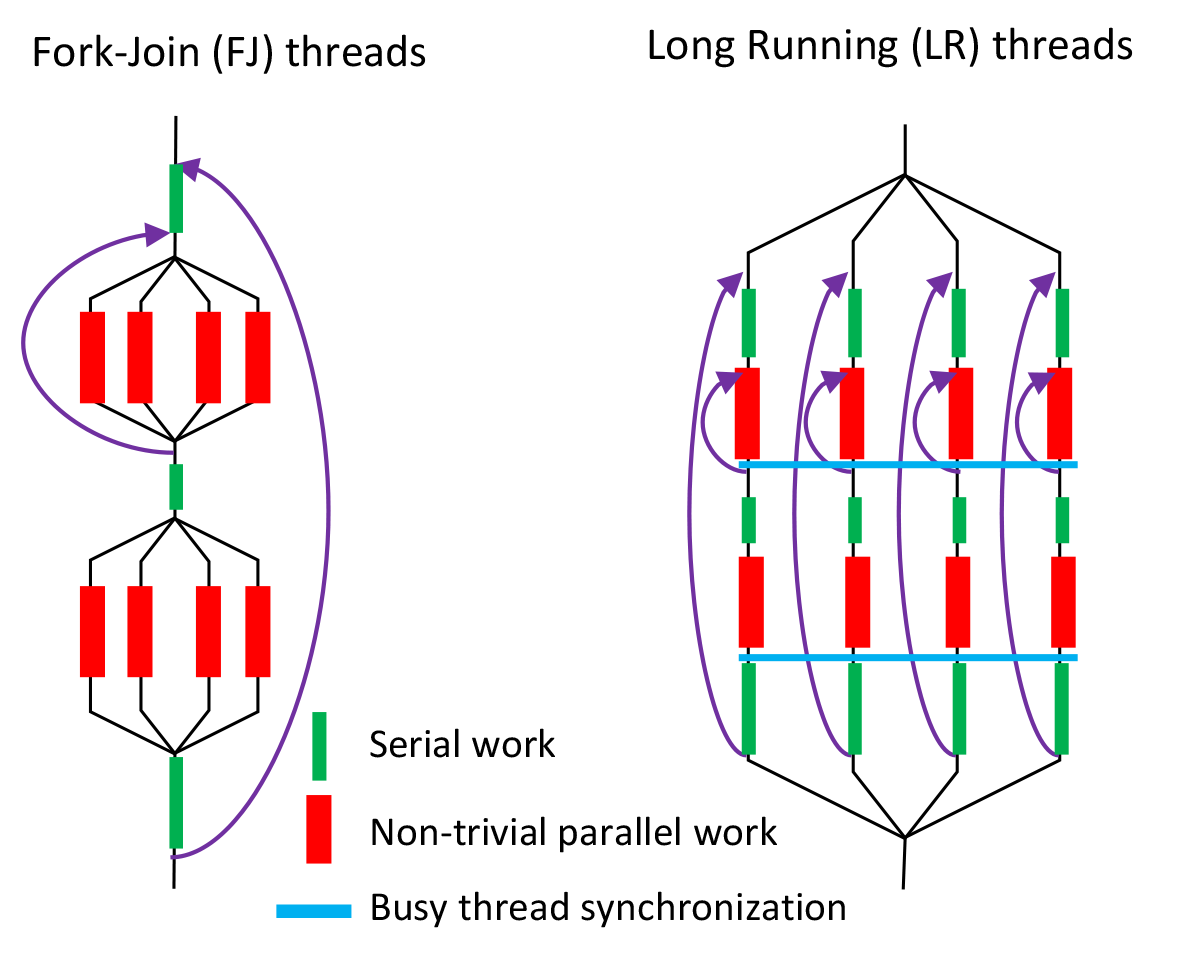
\includegraphics[width=0.8\columnwidth]{images/fig_fj_vs_lrt}
        \caption{Fork-Join vs. long running threads}
        \label{fig:fig_fj_vs_lrt}
    \end{minipage}
    \hspace{1.4mm}
    \begin{minipage}{0.49\textwidth}
        \centering
        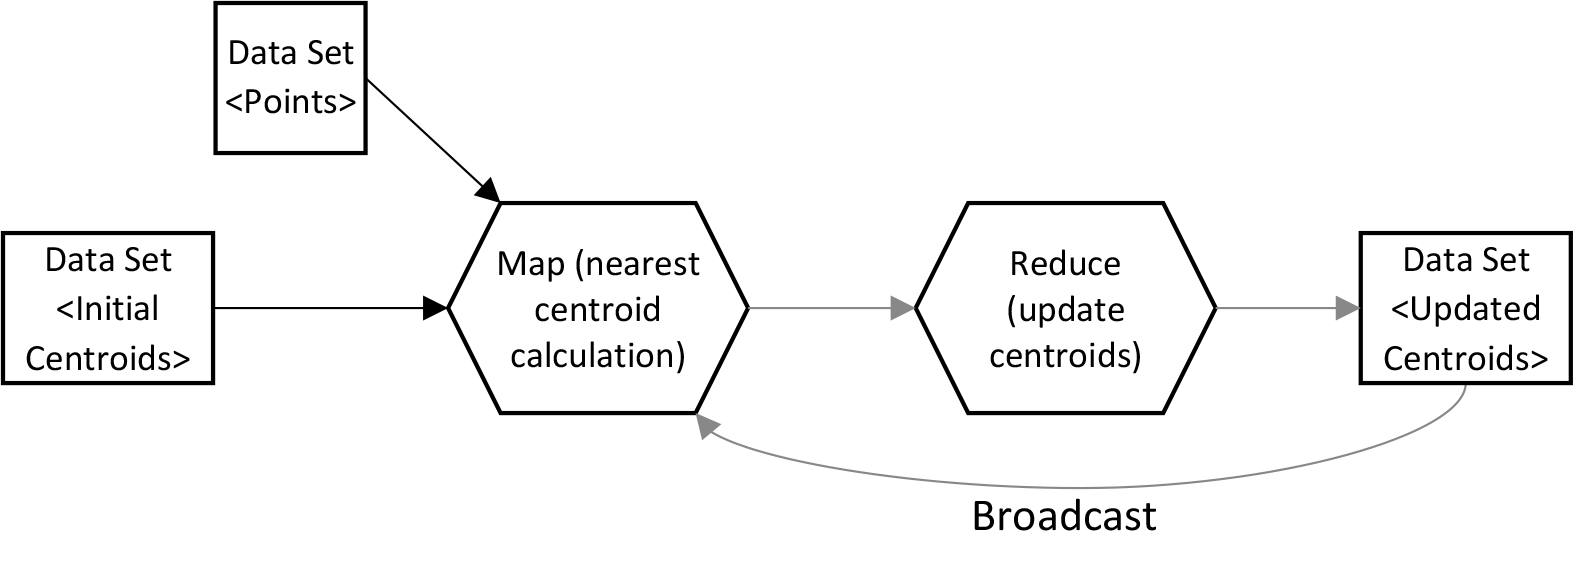
\includegraphics[width=1\columnwidth]{images/fig_kmeans_dataflow}
        \caption{Flink and Spark K-Means algorithm. Both Flink and Spark implementations follow the same data-flow}
        \label{fig:fig_flink_kmeans}
    \end{minipage}   
\end{figure*}

\section{Evaluation} \label{sec:evaluation}

%minipage kmeans Java and C 12 binding patterns
\begin{figure*}[!htb]
    \centering
    \begin{minipage}{.49\textwidth}
        \centering        
        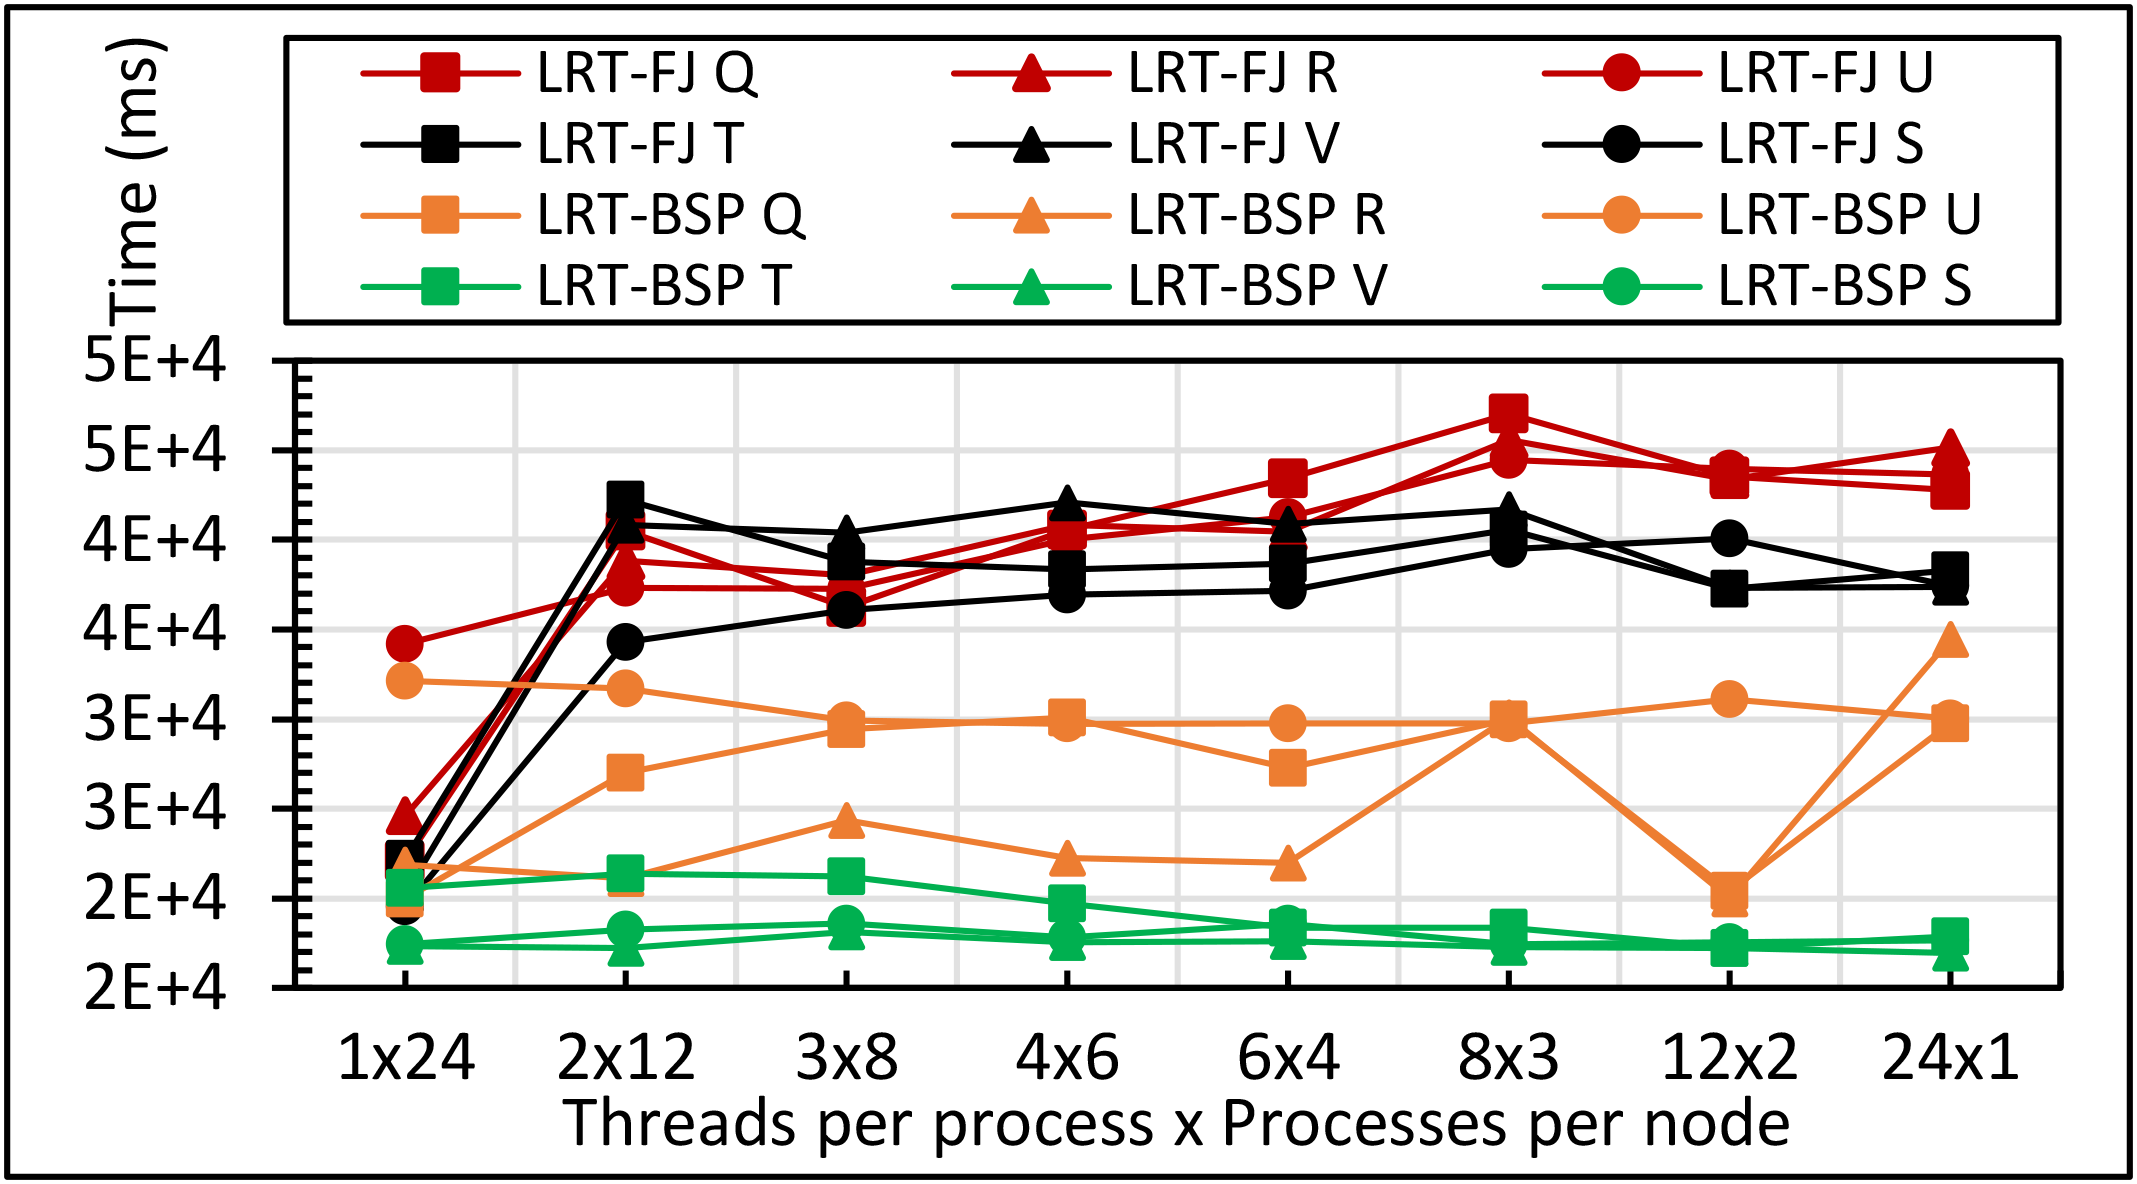
\includegraphics[width=1\columnwidth]{images/fig_kmeans_1mil_1k_binding_patterns}
        \caption{Java K-Means 1 mil points and 1k centers performance on 16 nodes for \ac{LRT-FJ} and \ac{LRT-BSP} with varying affinity patterns over varying threads and processes.}
        \label{fig:fig_kmeans_1mil_1k_binding_patterns}
    \end{minipage}
    \hspace{1.4mm}
    \begin{minipage}{0.49\textwidth}
        \centering
        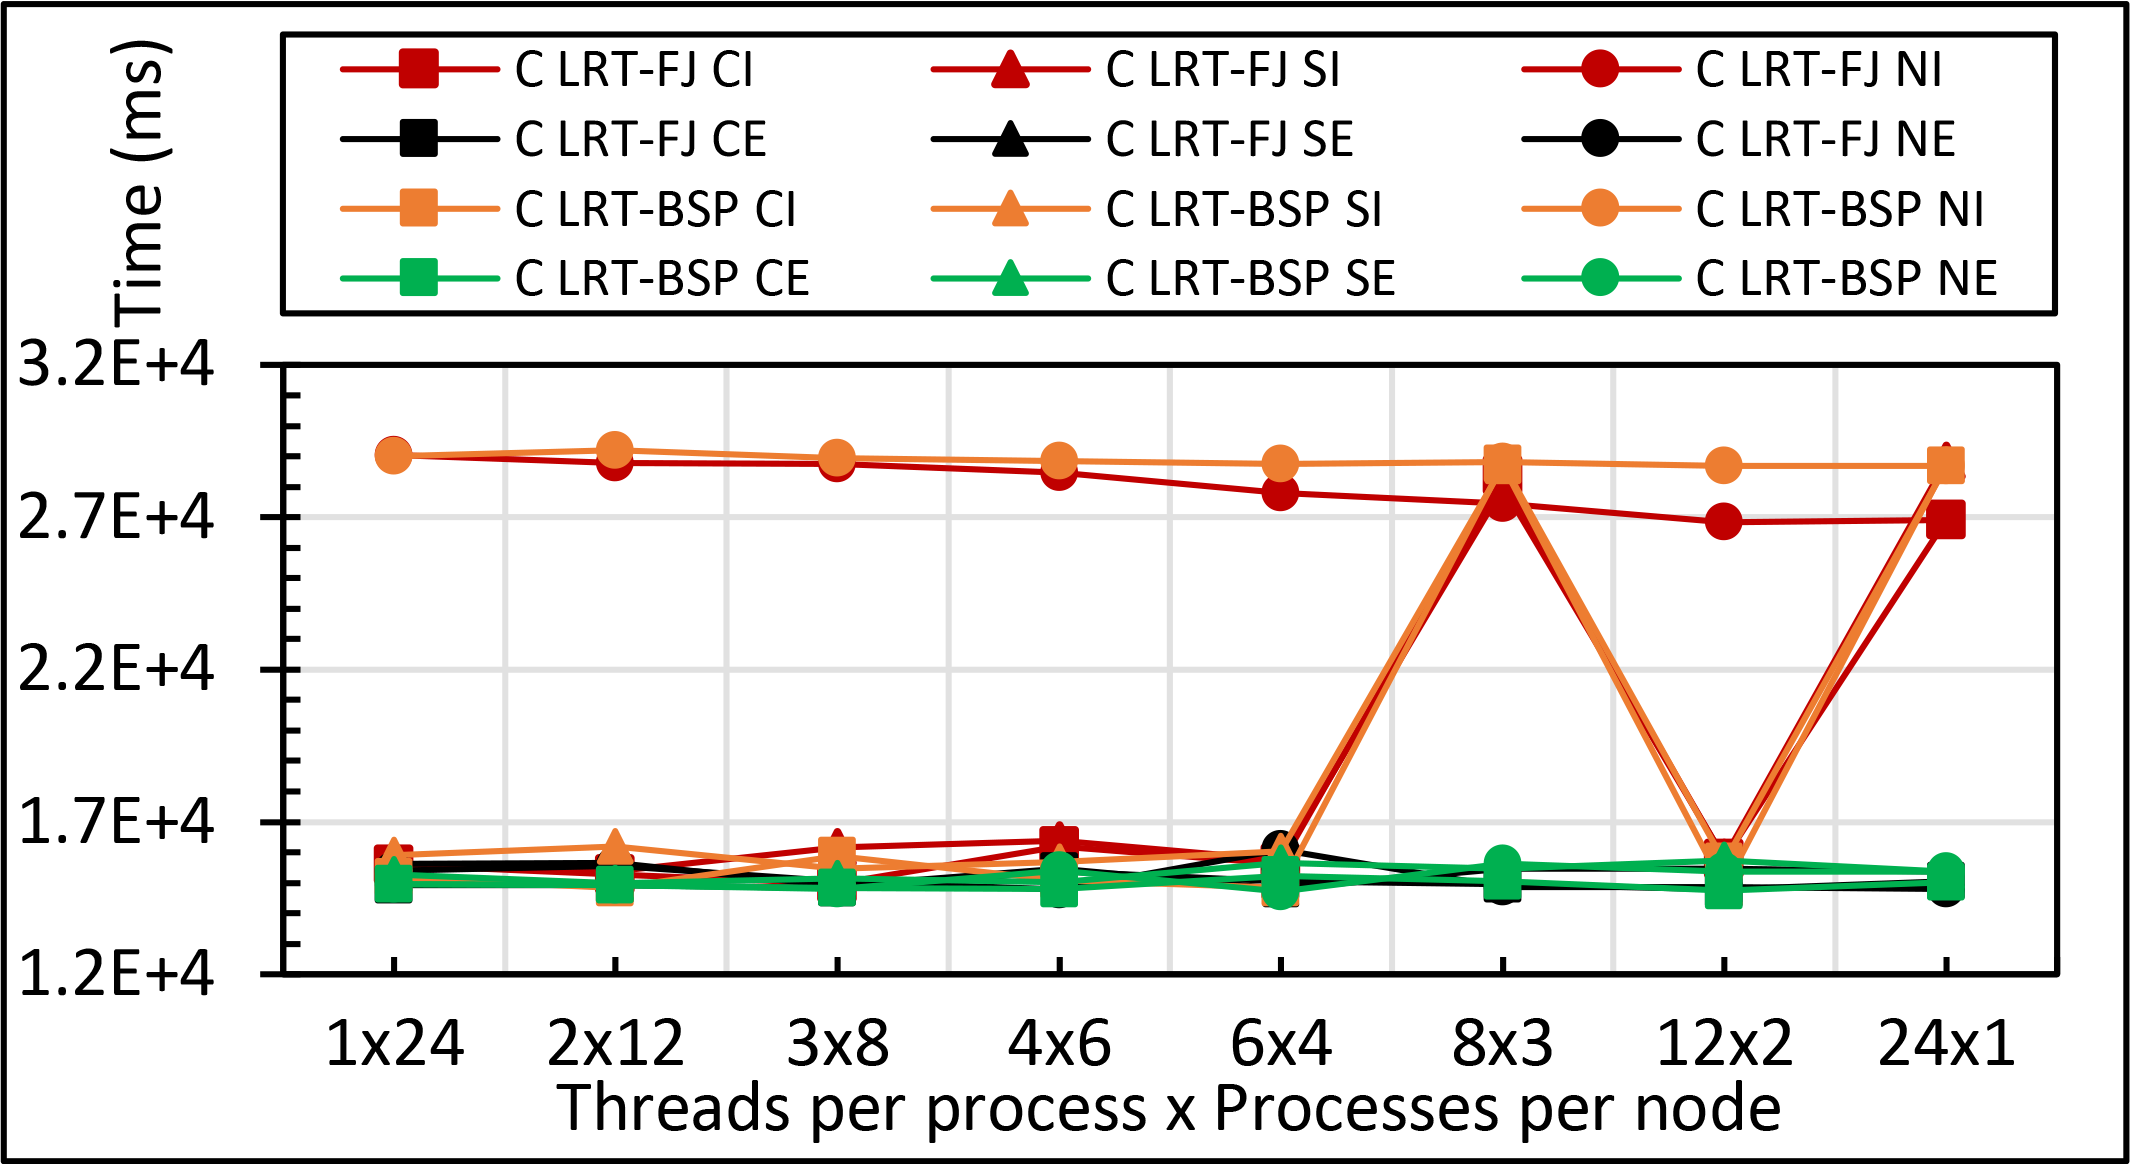
\includegraphics[width=1\columnwidth]{images/fig_C_kmeans_1mil_1k_binding_patterns}
        \caption{C K-Means 1 mil points and 1k centers performance on 16 nodes for \ac{LRT-FJ} and \ac{LRT-BSP} with varying affinity patterns over varying threads and processes.}
        \label{fig:fig_C_kmeans_1mil_1k_binding_patterns}
    \end{minipage}   
\end{figure*}

%minipage kmeans Java T vs S | Java vs C
\begin{figure*}[!htb]
    \begin{minipage}{0.49\textwidth}
        \centering
        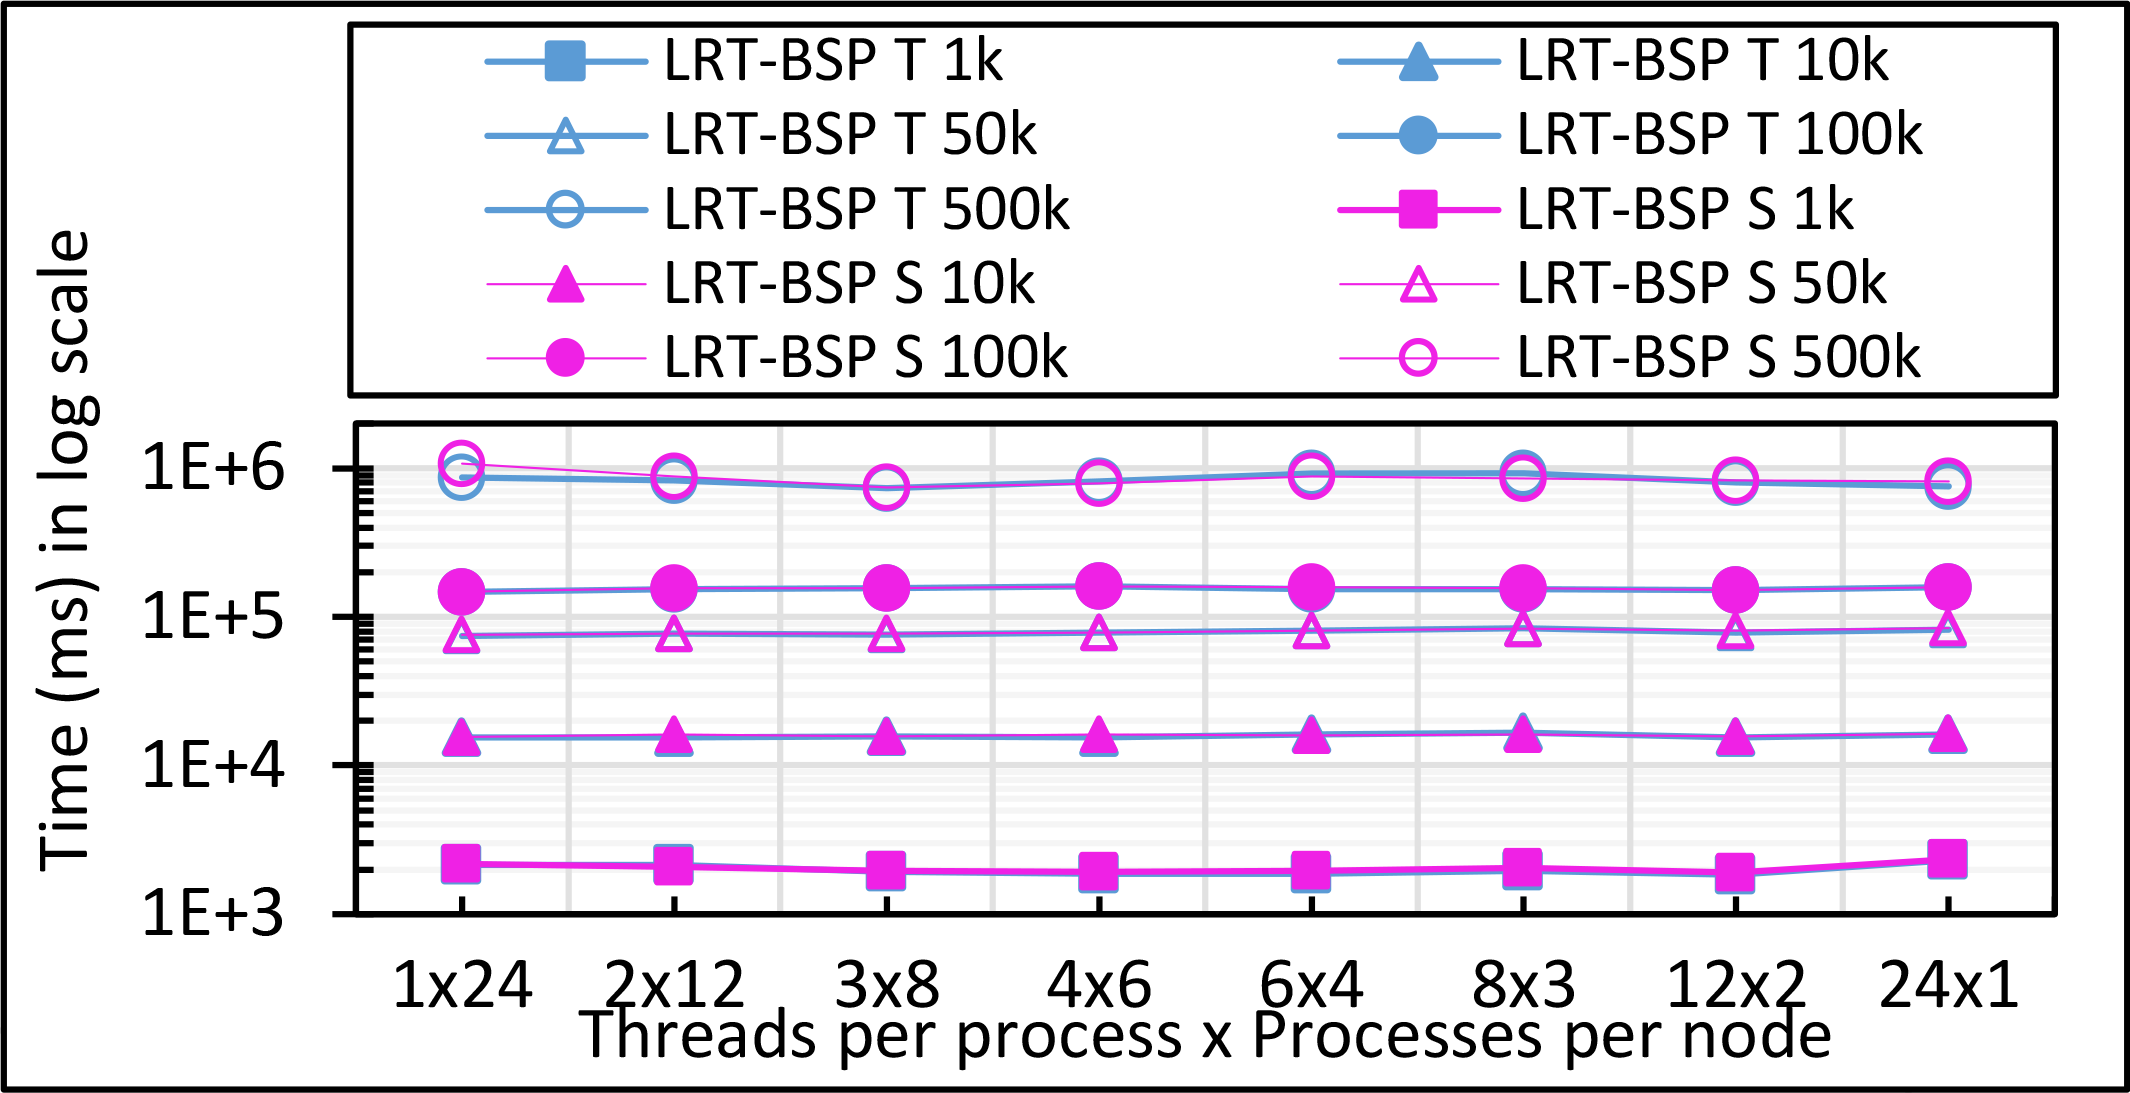
\includegraphics[width=1\columnwidth]{images/fig_kmeans_1mil_varying_centers_BSP_T_vs_BSP_S_Java}
		\caption{Java K-Means \ac{LRT-BSP} affinity T vs S performance for 1 mil points with 1k,10k,50k,100k, and 500k centers on 16 nodes over varying threads and processes.}
		\label{fig:images/fig_kmeans_1mil_varying_centers_BSP_T_vs_BSP_S_Java}
    \end{minipage}
    \hspace{1.4mm}
    \begin{minipage}{0.49\textwidth}
        \centering
        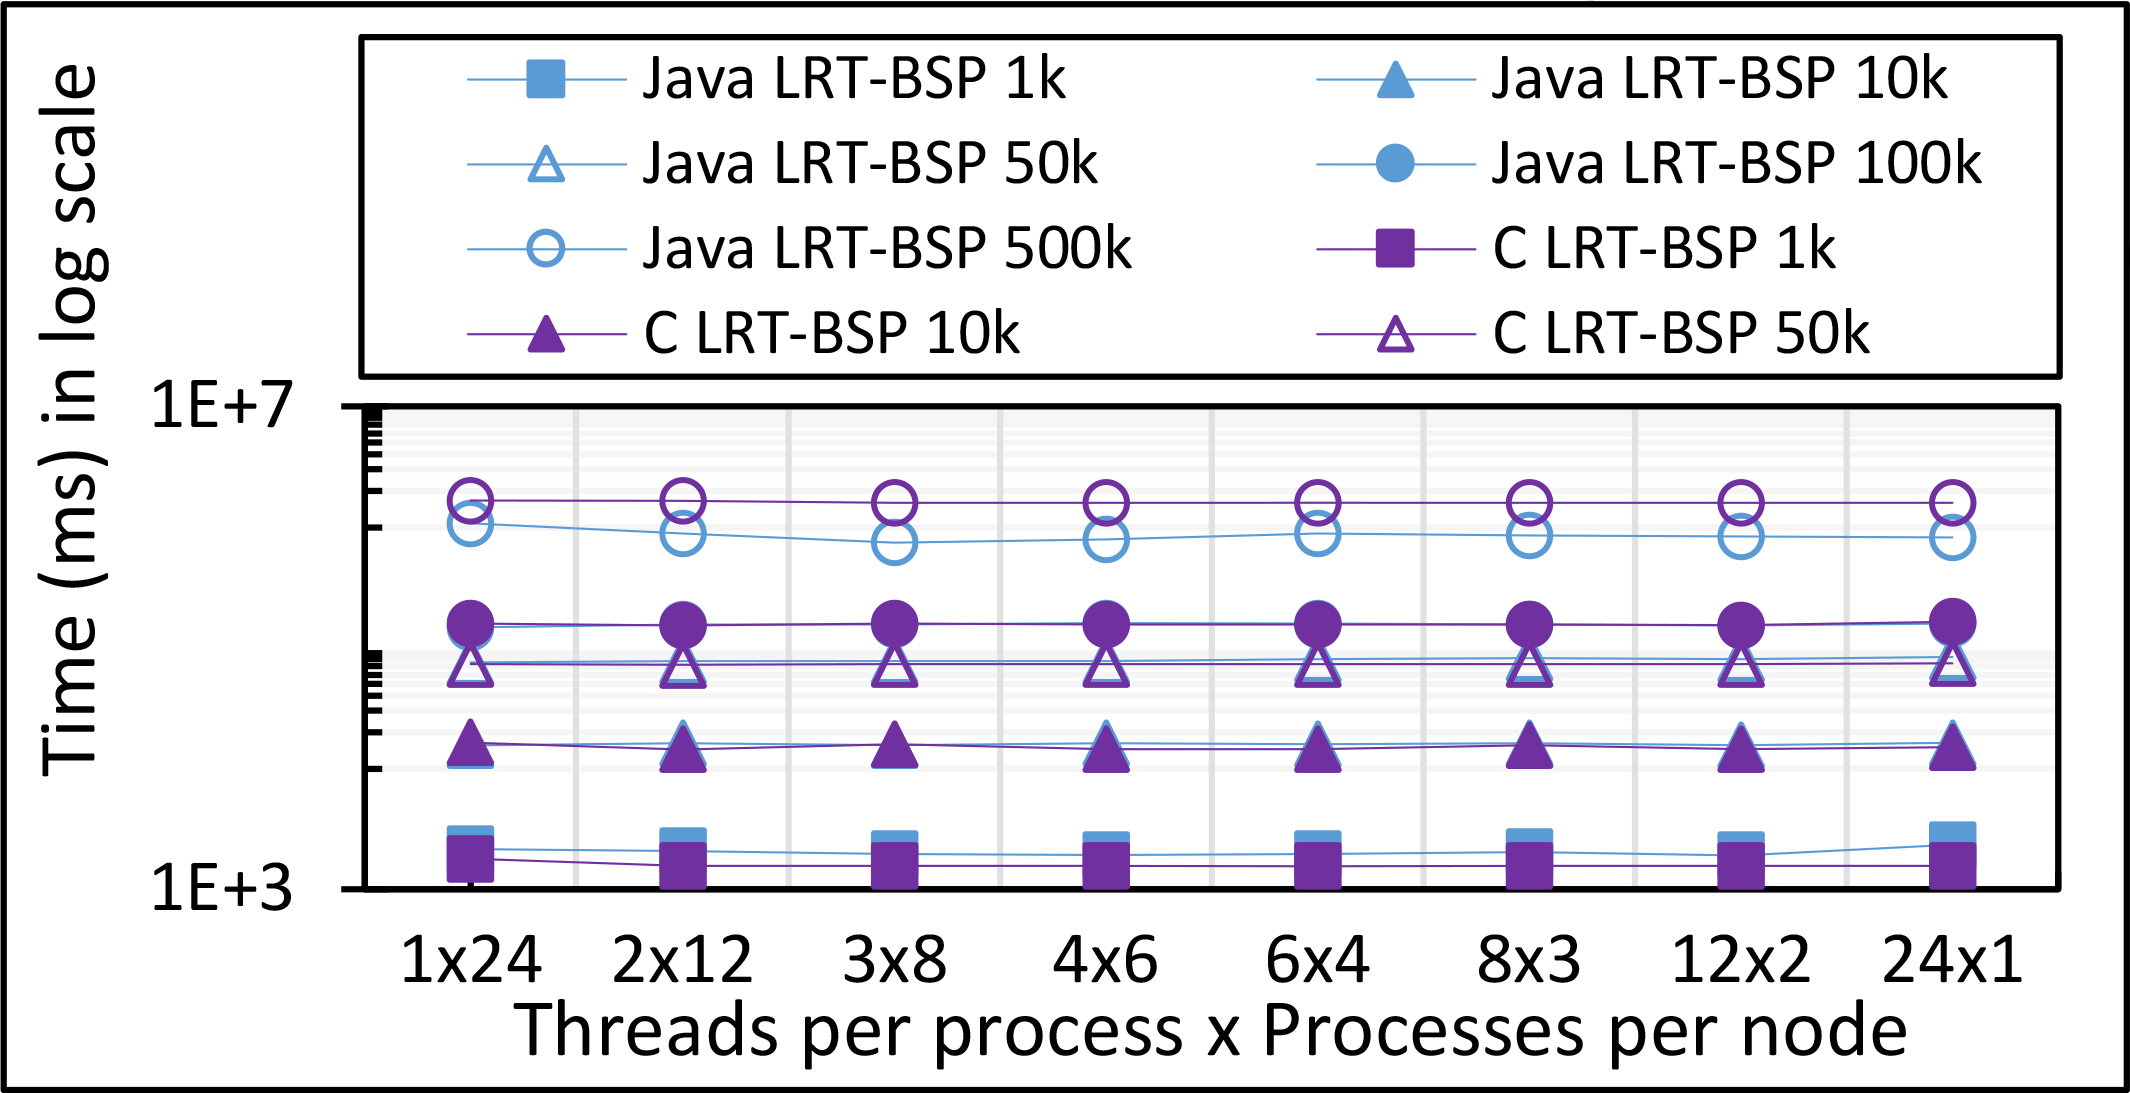
\includegraphics[width=1\columnwidth]{images/fig_kmeans_1mil_varying_centers_BSP_T_C_vs_Java}
		\caption{Java vs C K-Means \ac{LRT-BSP} affinity T performance for 1 mil points with 1k,10k,50k,100k, and 500k centers on 16 nodes over varying threads and processes.}
		\label{fig:images/fig_kmeans_1mil_varying_centers_BSP_T_C_vs_Java}
    \end{minipage}   
\end{figure*}

%minipage kmeans 1k,10k,100k | 50k 500k 
\begin{figure*}[!htb]
	\begin{minipage}{0.49\textwidth}
        \centering
        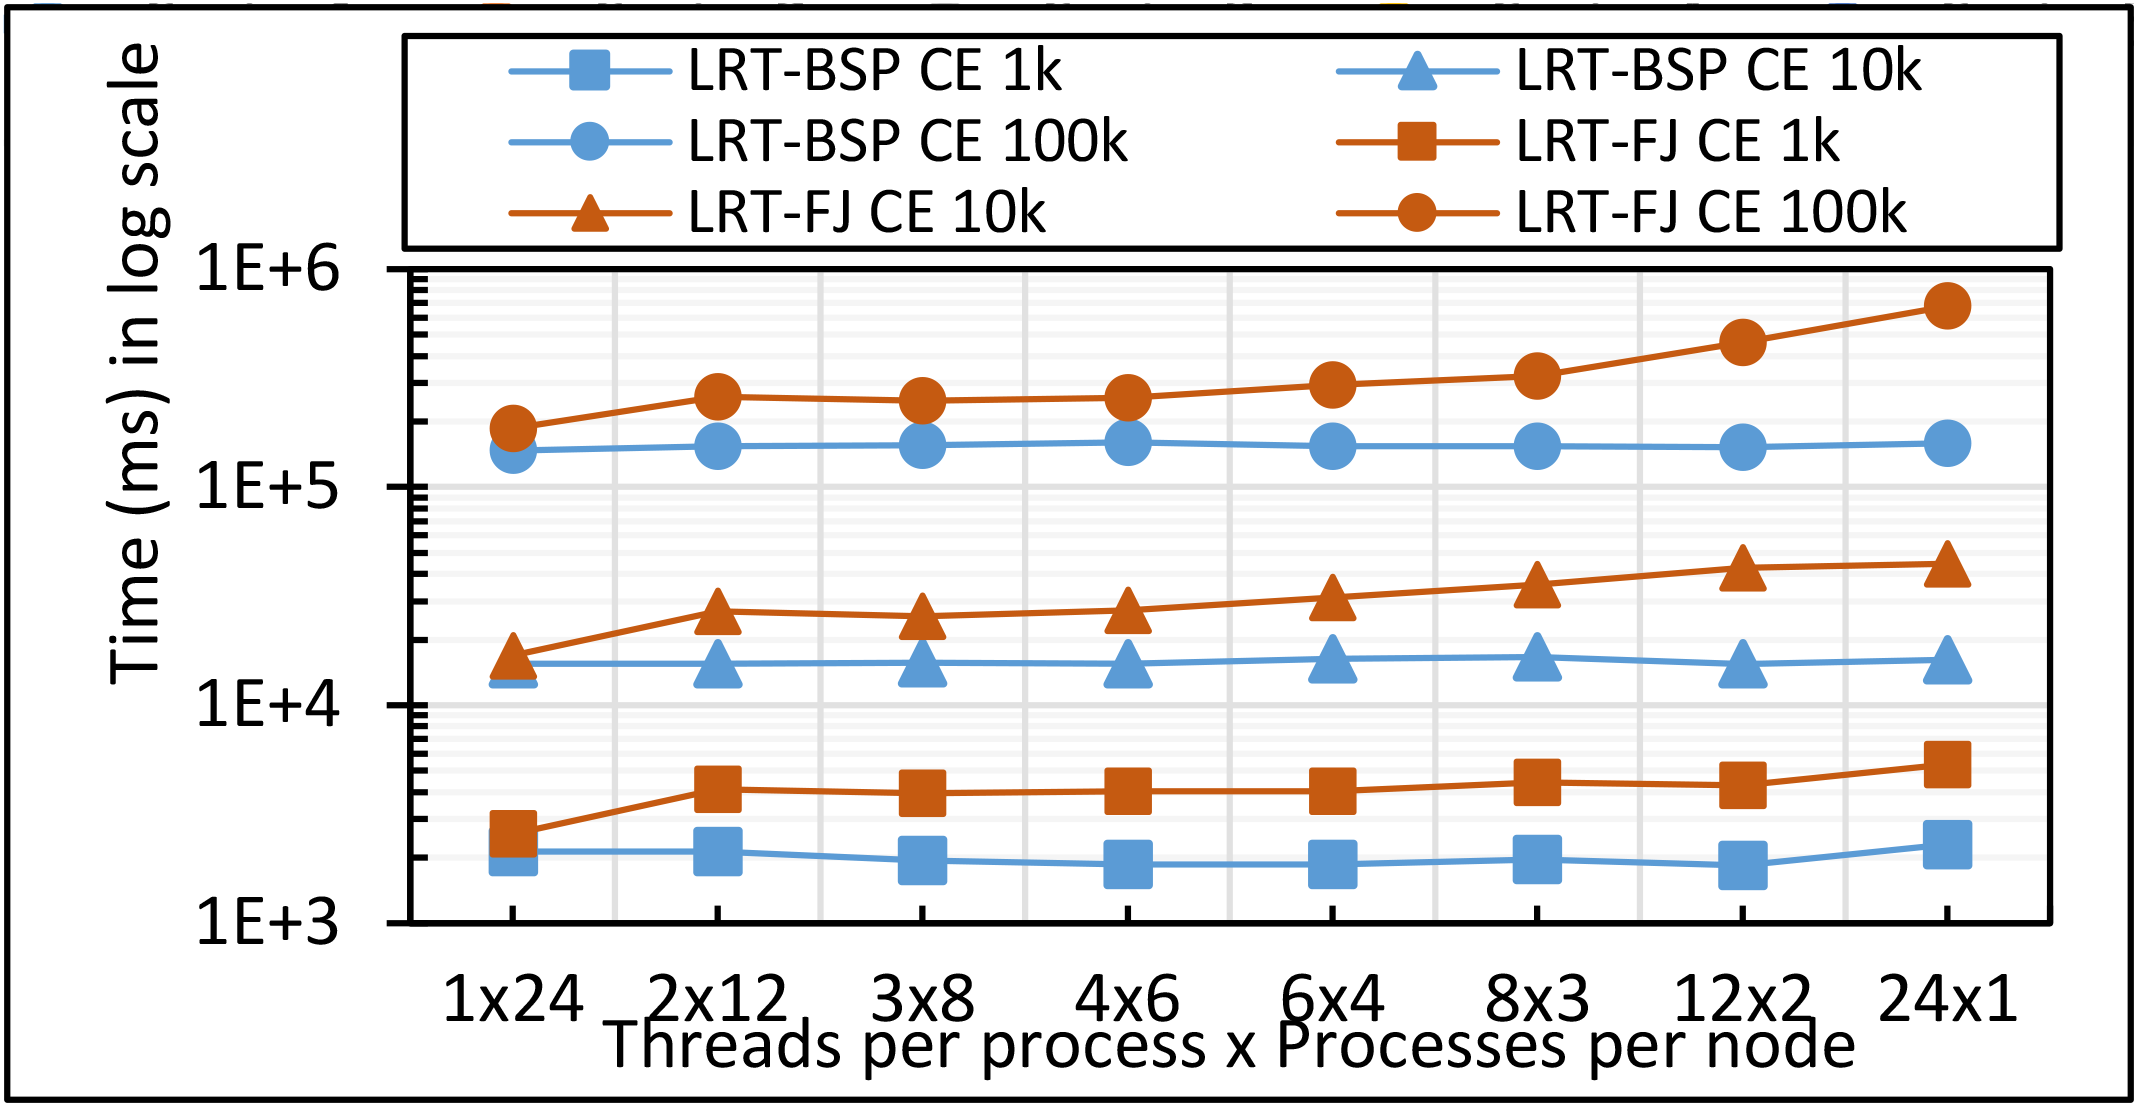
\includegraphics[width=1\columnwidth]{images/fig_kmeans_1mil_varying_centers_by_10k_FJ_vs_BSP_T}
        \caption{Java K-Means 1 mil points with 1k,10k, and 100k centers performance on 16 nodes for \ac{LRT-FJ} and \ac{LRT-BSP} over varying threads and processes. The affinity pattern is T.}
        \label{fig:fig_kmeans_1mil_varying_centers_by_10k_FJ_vs_BSP_T}
    \end{minipage}
    \hspace{1.4mm}
    \begin{minipage}{0.49\textwidth}
        \centering
        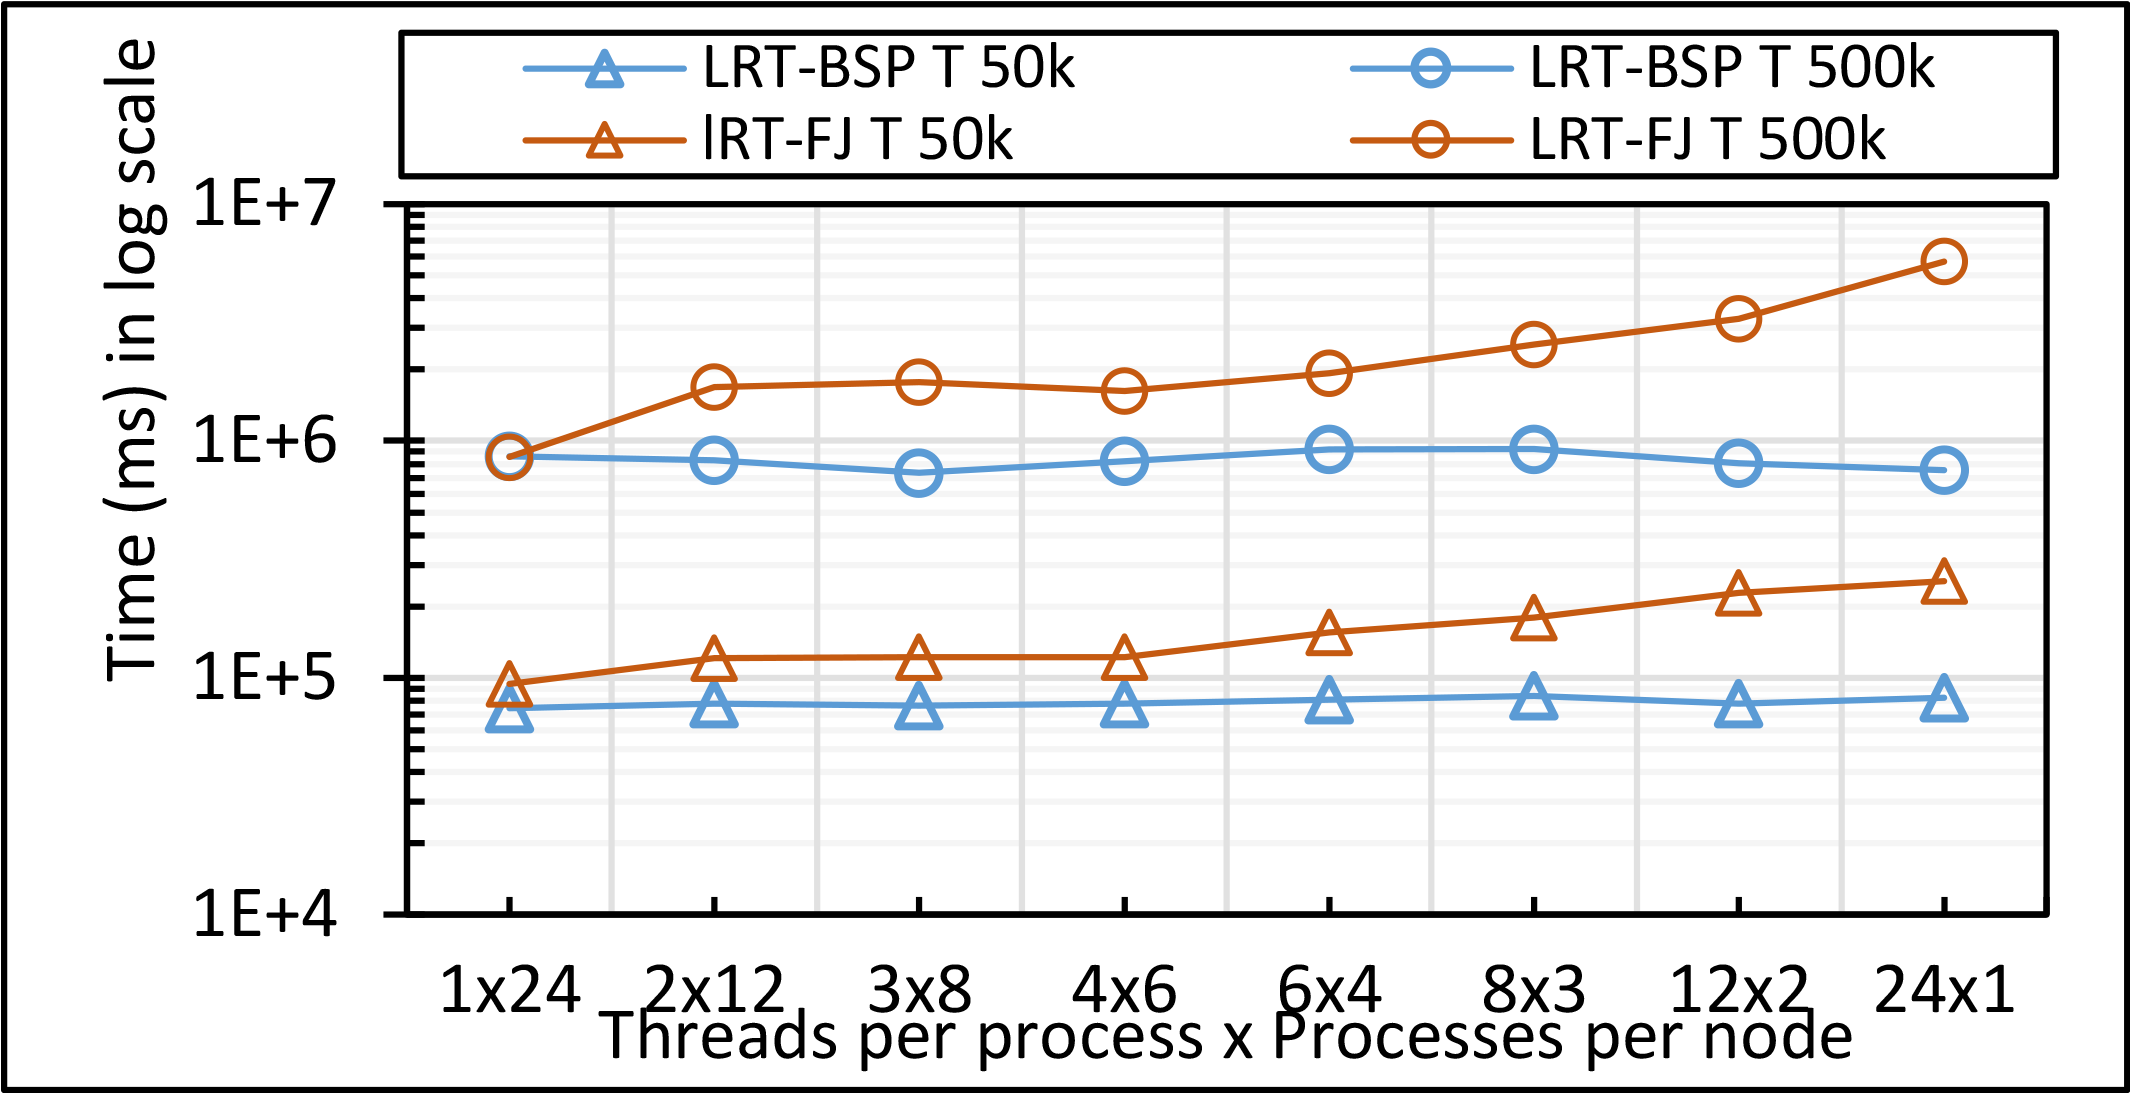
\includegraphics[width=1\columnwidth]{images/fig_kmeans_1mil_varying_centers_as_50k_500k_FJ_vs_BSP_T}
        \caption{Java K-Means 1 mil points with 50k, and 500k centers performance on 16 nodes for \ac{LRT-FJ} and \ac{LRT-BSP} over varying threads and processes. The affinity pattern is T.}
        \label{fig:fig_kmeans_1mil_varying_centers_as_50k_500k_FJ_vs_BSP_T}
    \end{minipage}
\end{figure*}

%minipage damds 50k 24core and 36core
\begin{figure*}[!htb]
	\begin{minipage}{0.49\textwidth}
        \centering
        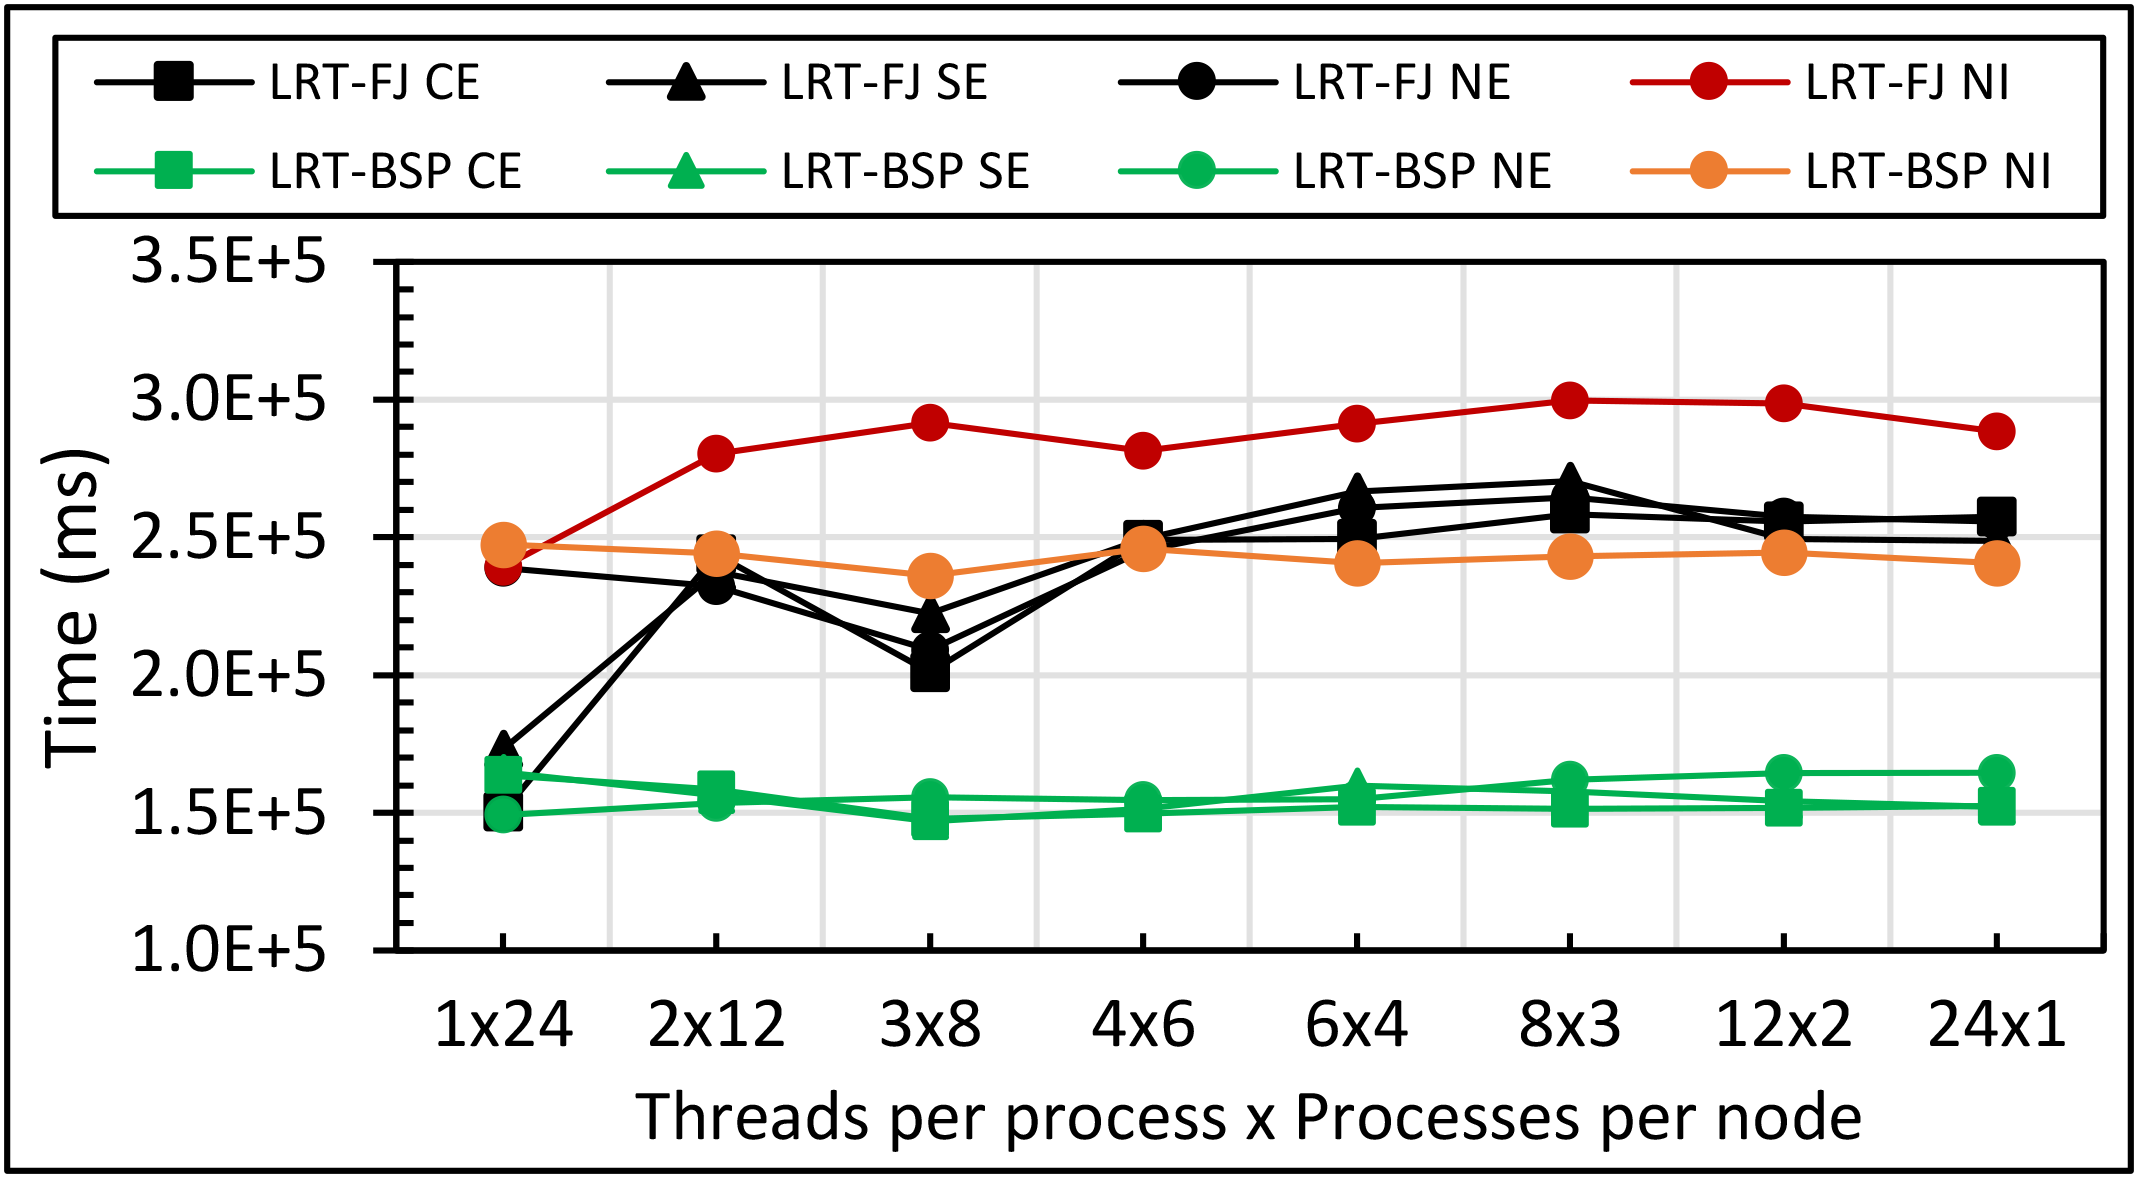
\includegraphics[width=1\columnwidth]{images/fig_damds_50k_binding_patterns}
        \caption{Java DA-MDS 50k points performance on 16 nodes for \ac{LRT-FJ} and \ac{LRT-BSP} over varying threads and processes. Affinity patterns are T,S,V, and U.}
        \label{fig:fig_damds_50k_binding_patterns}
    \end{minipage}
    \hspace{1.4mm}
    \begin{minipage}{0.49\textwidth}
        \centering
        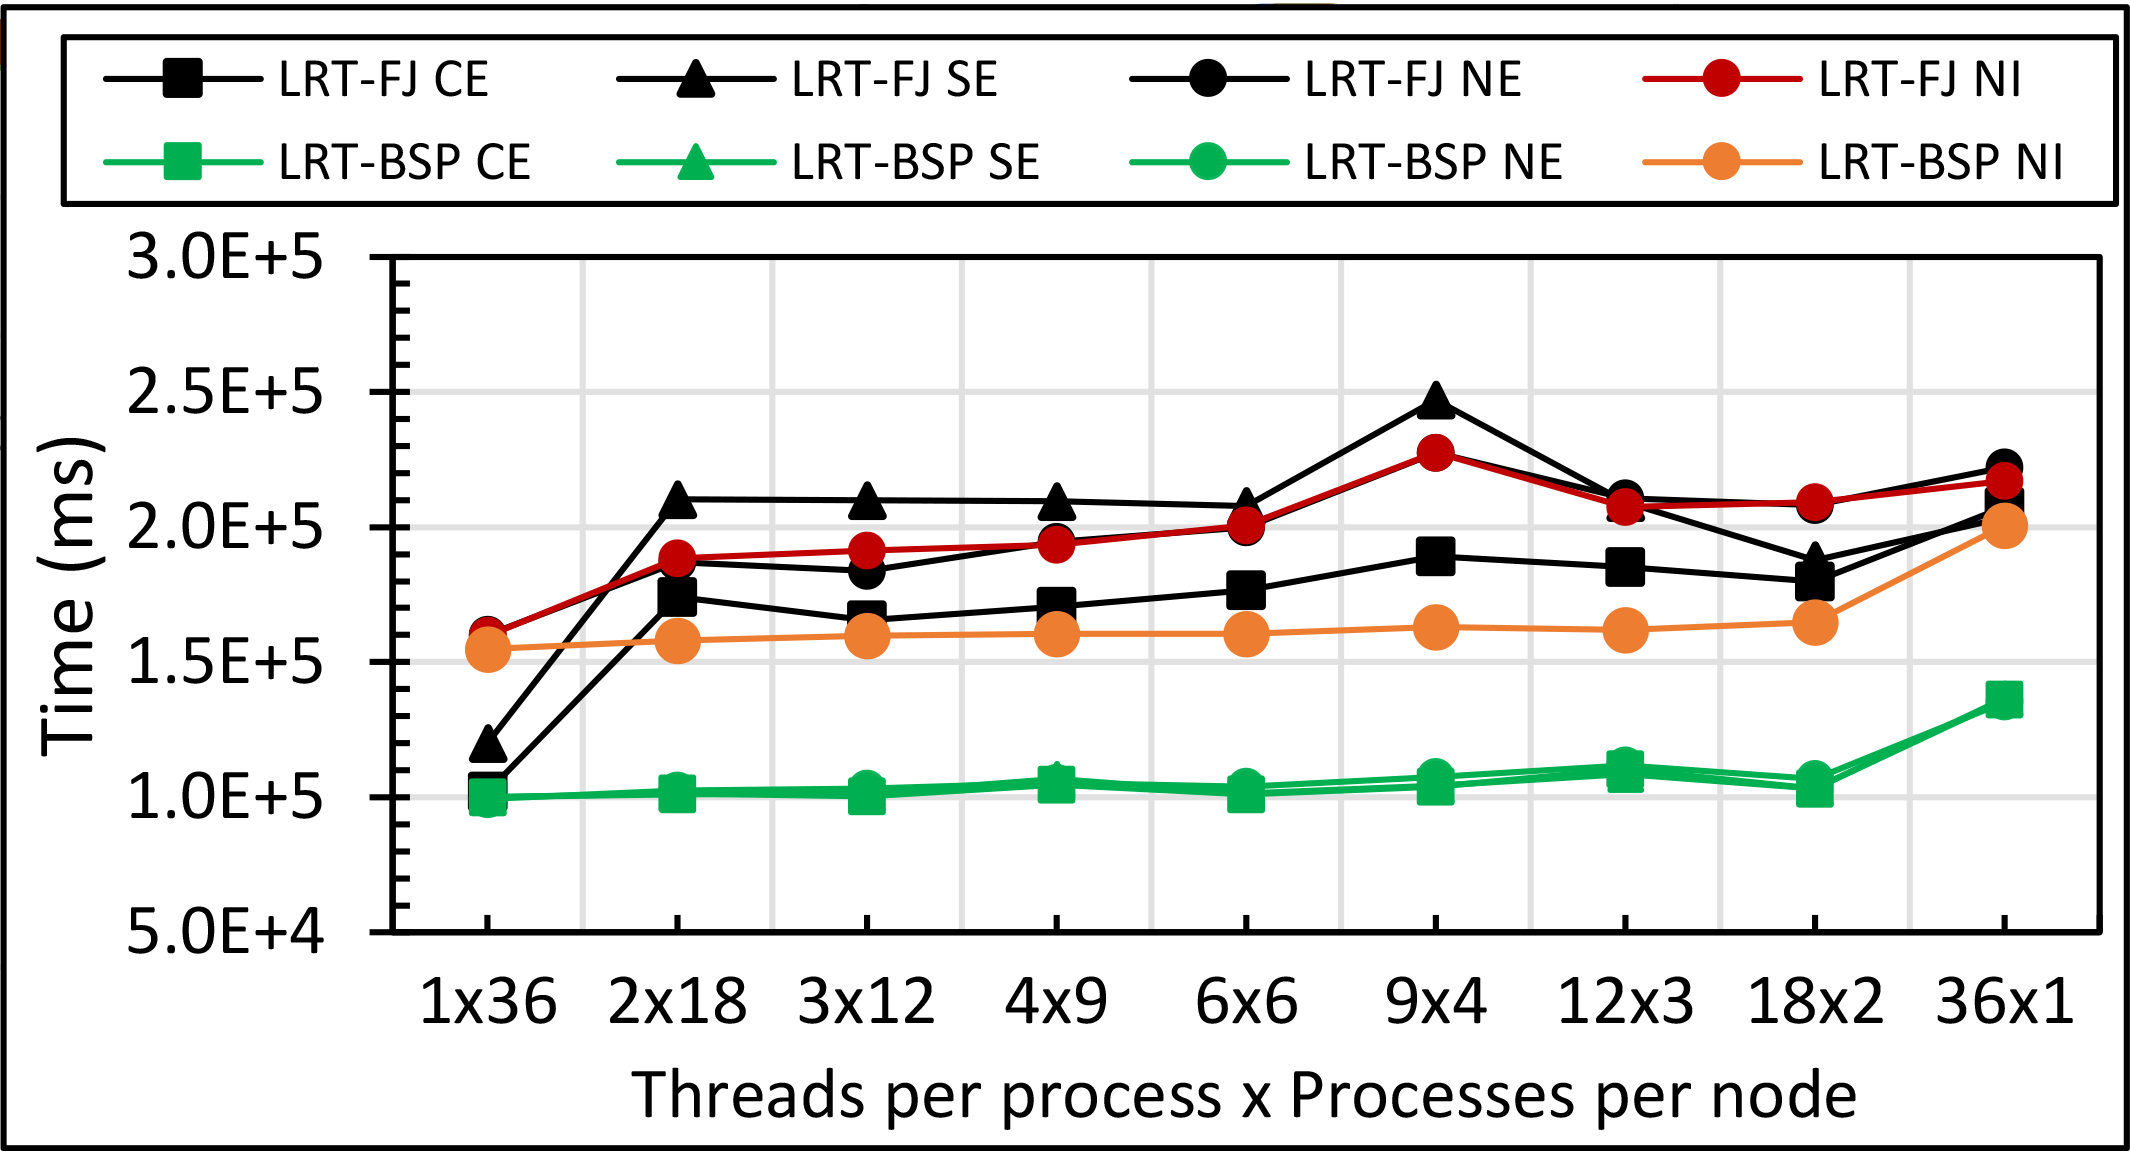
\includegraphics[width=1\columnwidth]{images/fig_damds_50k_binding_patterns_on_36core_nodes}
        \caption{Java DA-MDS 50k points performance on 16 of 36-core nodes for \ac{LRT-FJ} and \ac{LRT-BSP} over varying threads and processes. Affinity patterns are T,S,V, and U.}
        \label{fig:fig_damds_50k_binding_patterns_on_36core_nodes}
    \end{minipage}
\end{figure*}

%minipage damds 100k 24core and 36core
\begin{figure*}[!htb]
	\begin{minipage}{0.49\textwidth}
        \centering
        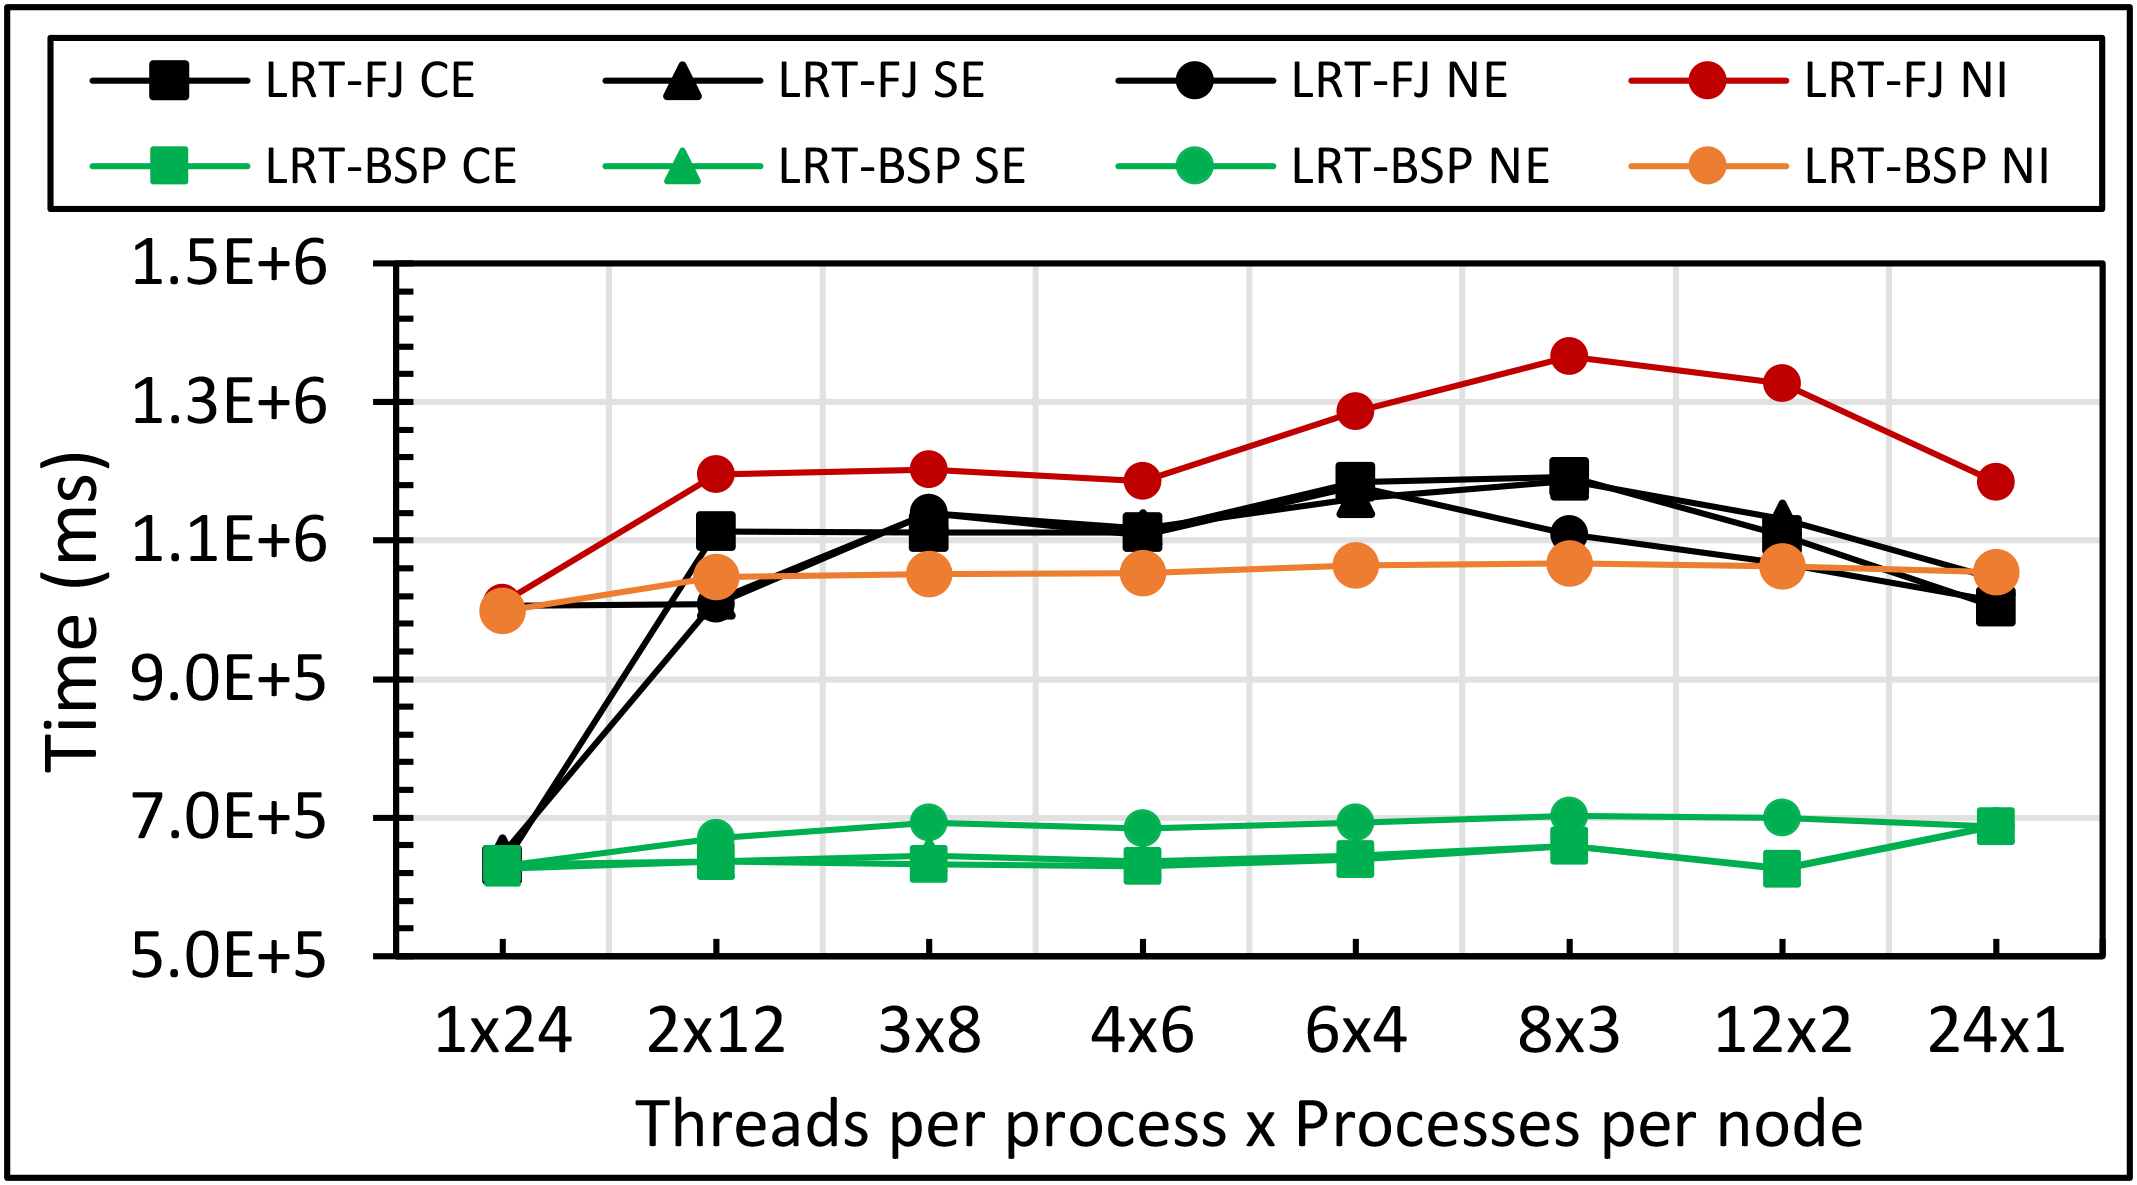
\includegraphics[width=1\columnwidth]{images/fig_damds_100k_binding_patterns}
        \caption{Java DA-MDS 100k points performance on 16 nodes for \ac{LRT-FJ} and \ac{LRT-BSP} over varying threads and processes. Affinity patterns are T,S,V, and U.}
        \label{fig:fig_damds_100k_binding_patterns}
    \end{minipage}
    \hspace{1.4mm}
    \begin{minipage}{0.49\textwidth}
        \centering
        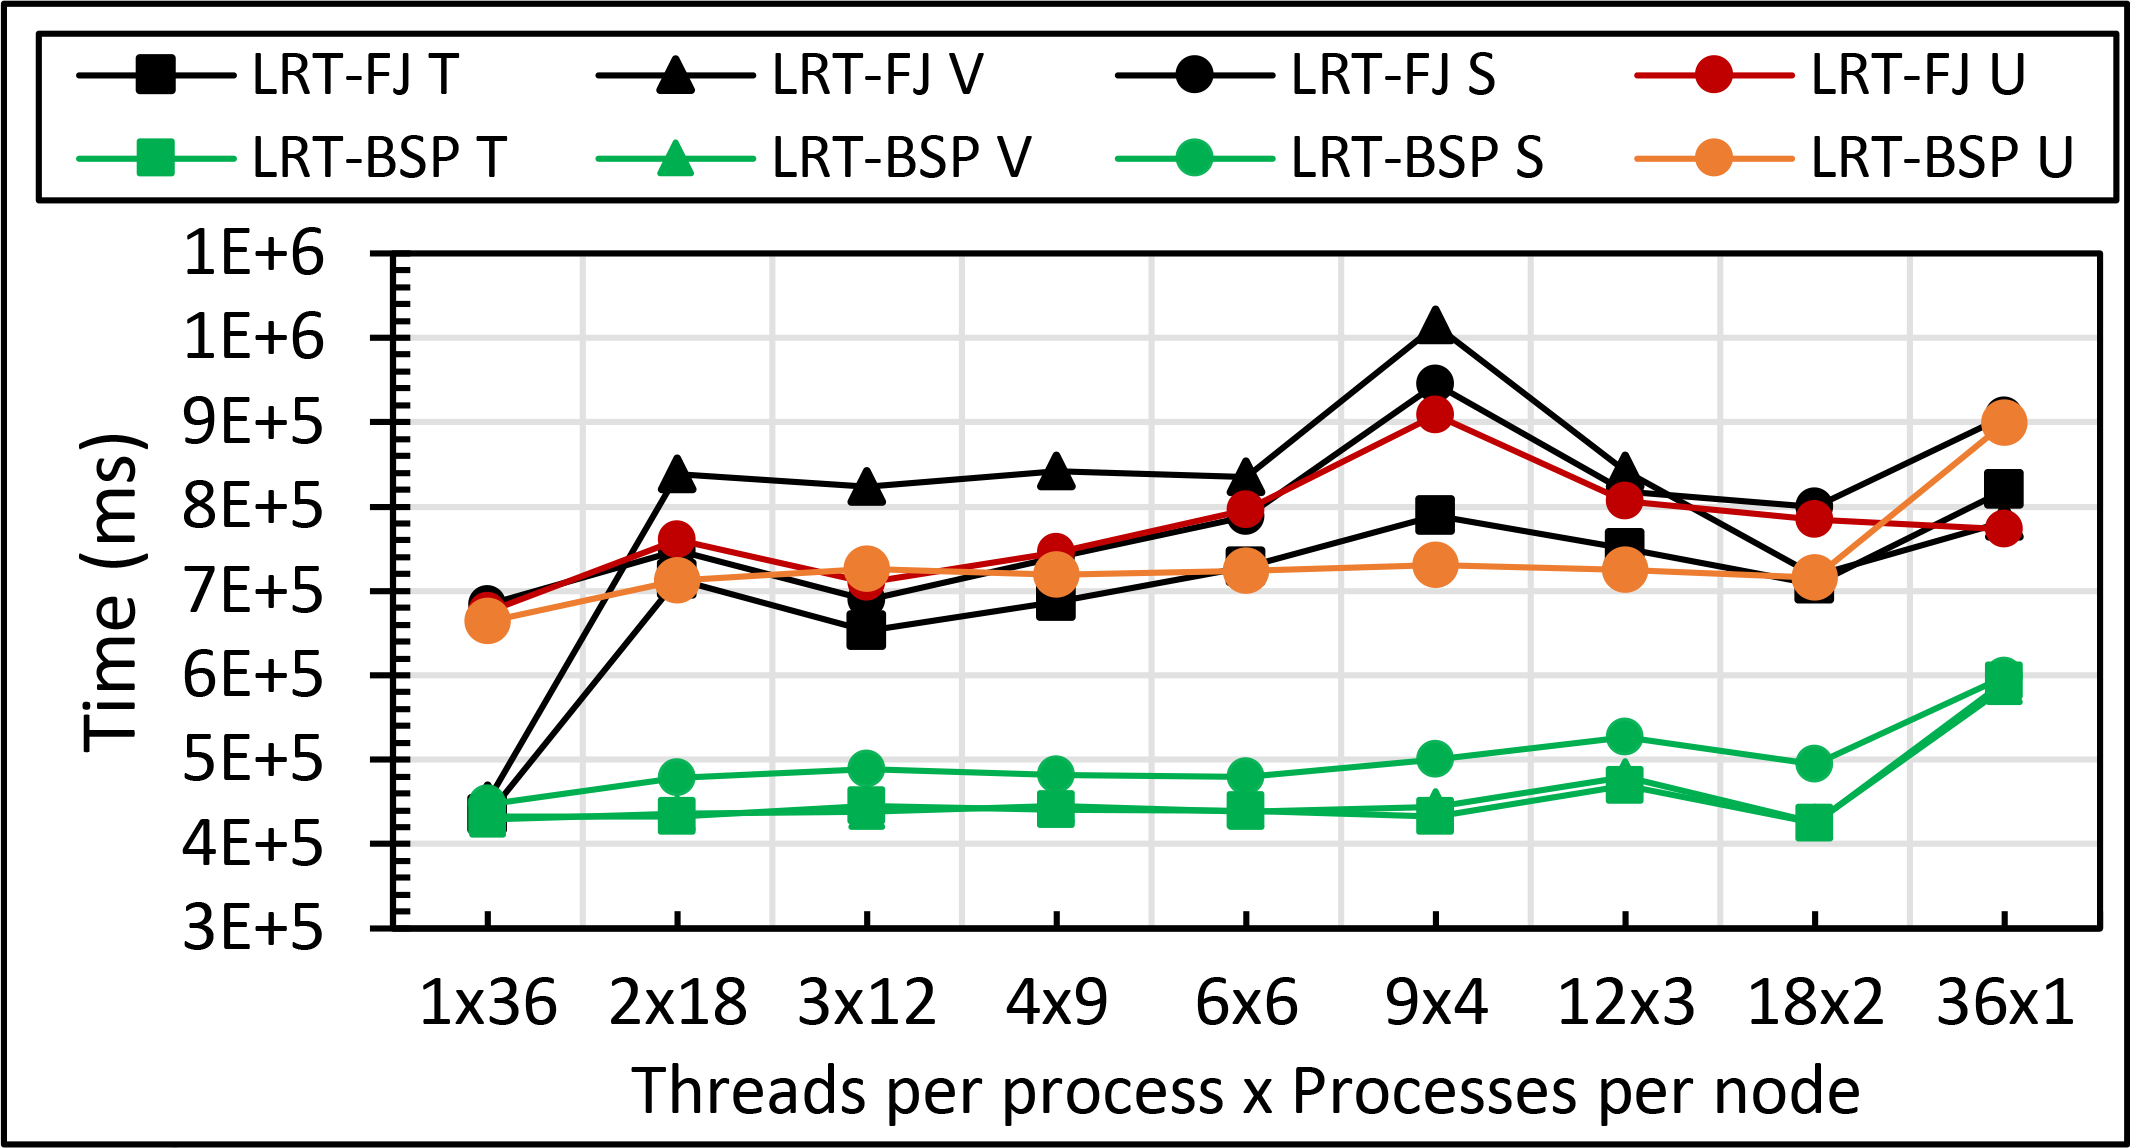
\includegraphics[width=1\columnwidth]{images/fig_damds_100k_binding_patterns_on_36core_nodes}
        \caption{Java DA-MDS 100k points performance on 16 of 36-core nodes for \ac{LRT-FJ} and \ac{LRT-BSP} over varying threads and processes. Affinity patterns are T,S,V, and U.}
        \label{fig:fig_damds_100k_binding_patterns_on_36core_nodes}
    \end{minipage}
\end{figure*}

%minipage damds 200k 24core and 36core
\begin{figure*}[!htb]
	\begin{minipage}{0.49\textwidth}
        \centering
        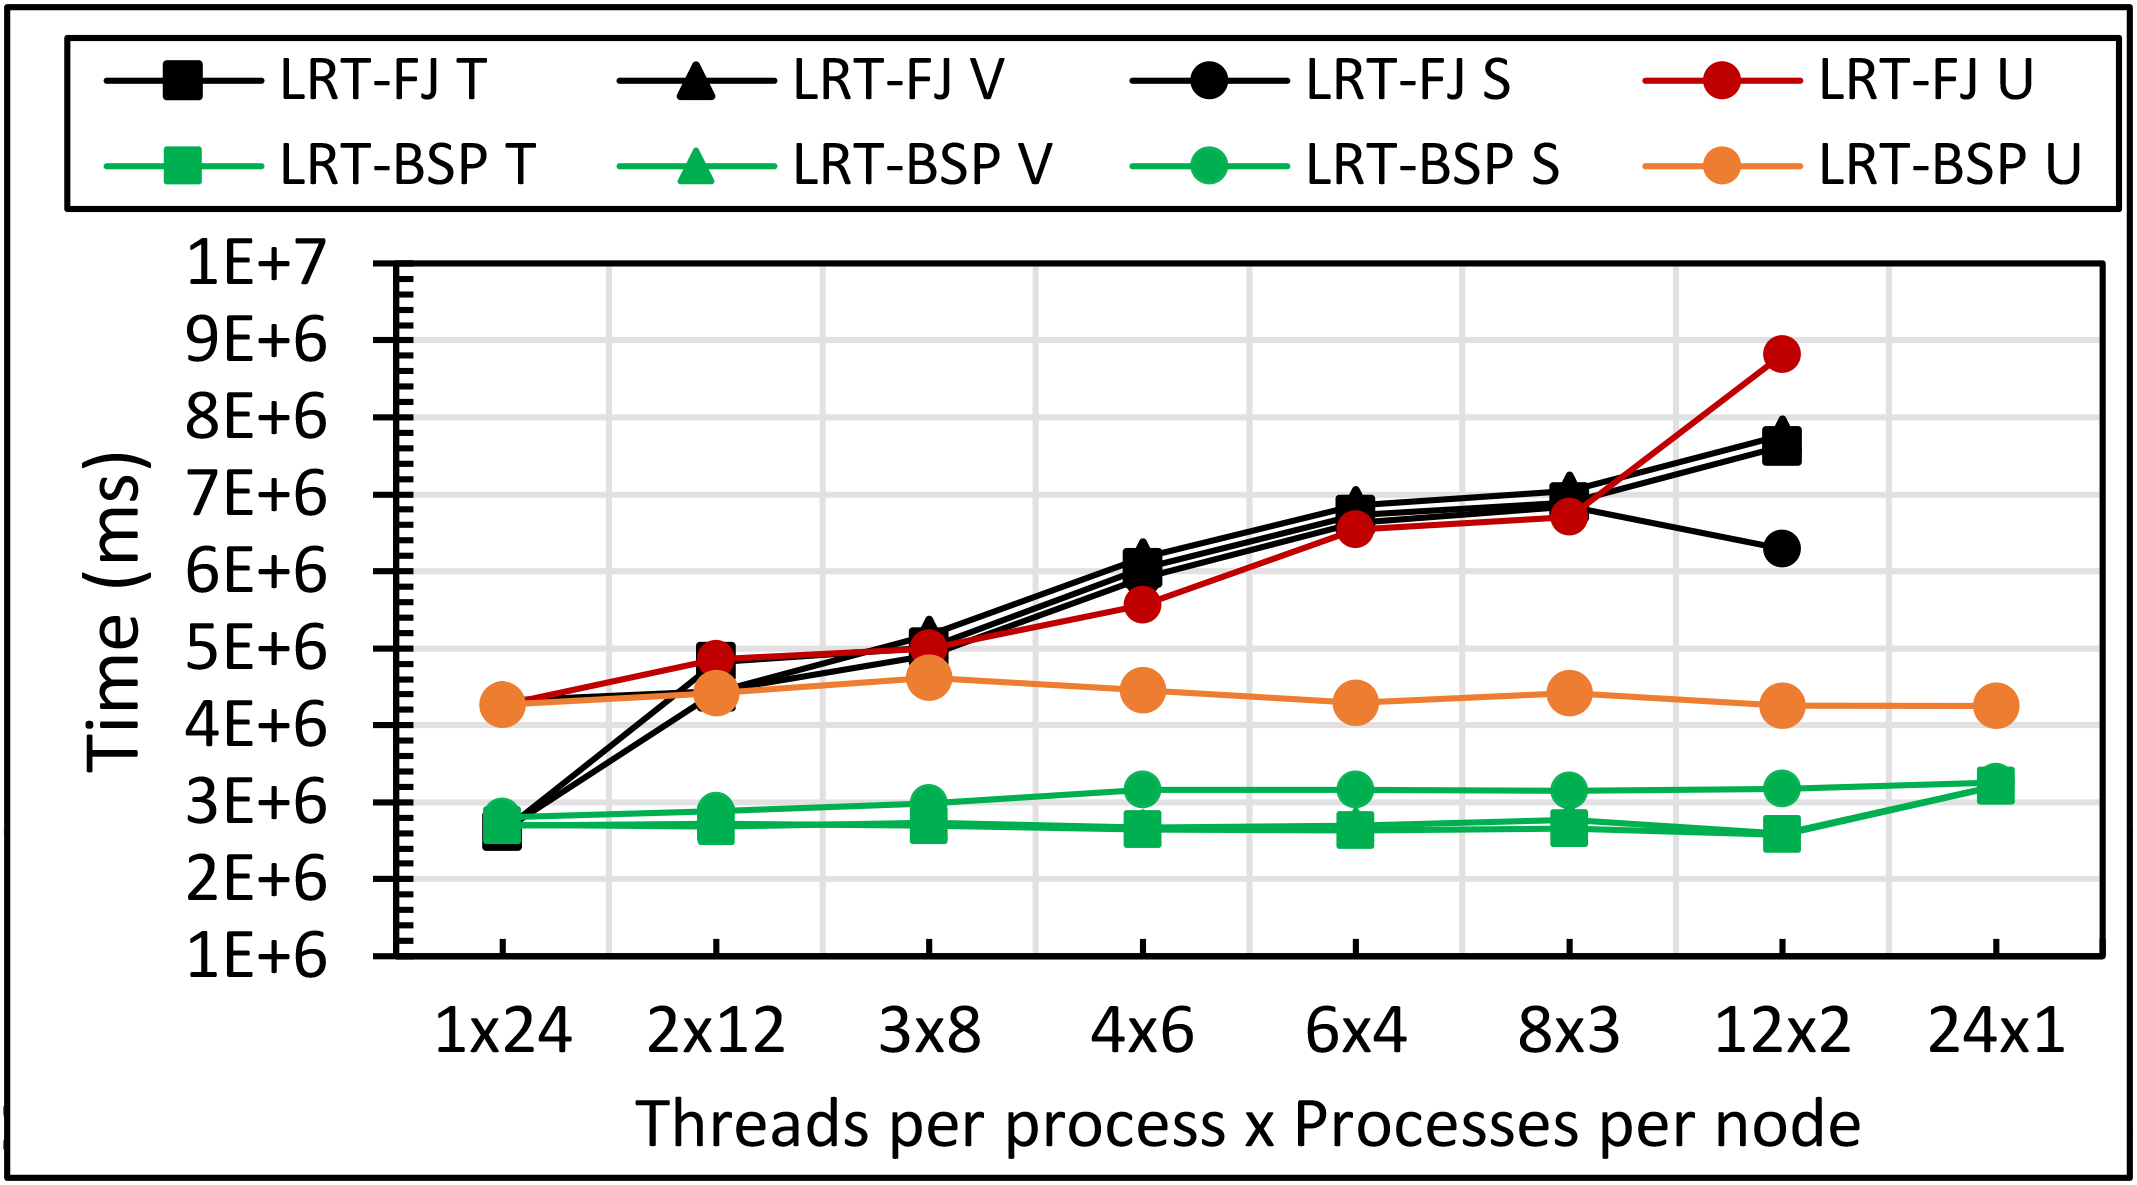
\includegraphics[width=1\columnwidth]{images/fig_damds_200k_binding_patterns}
        \caption{Java DA-MDS 200k points performance on 16 nodes for \ac{LRT-FJ} and \ac{LRT-BSP} over varying threads and processes. Affinity patterns are T,S,V, and U.}
        \label{fig:fig_damds_200k_binding_patterns}
    \end{minipage}
    \hspace{1.4mm}
    \begin{minipage}{0.49\textwidth}
        \centering
        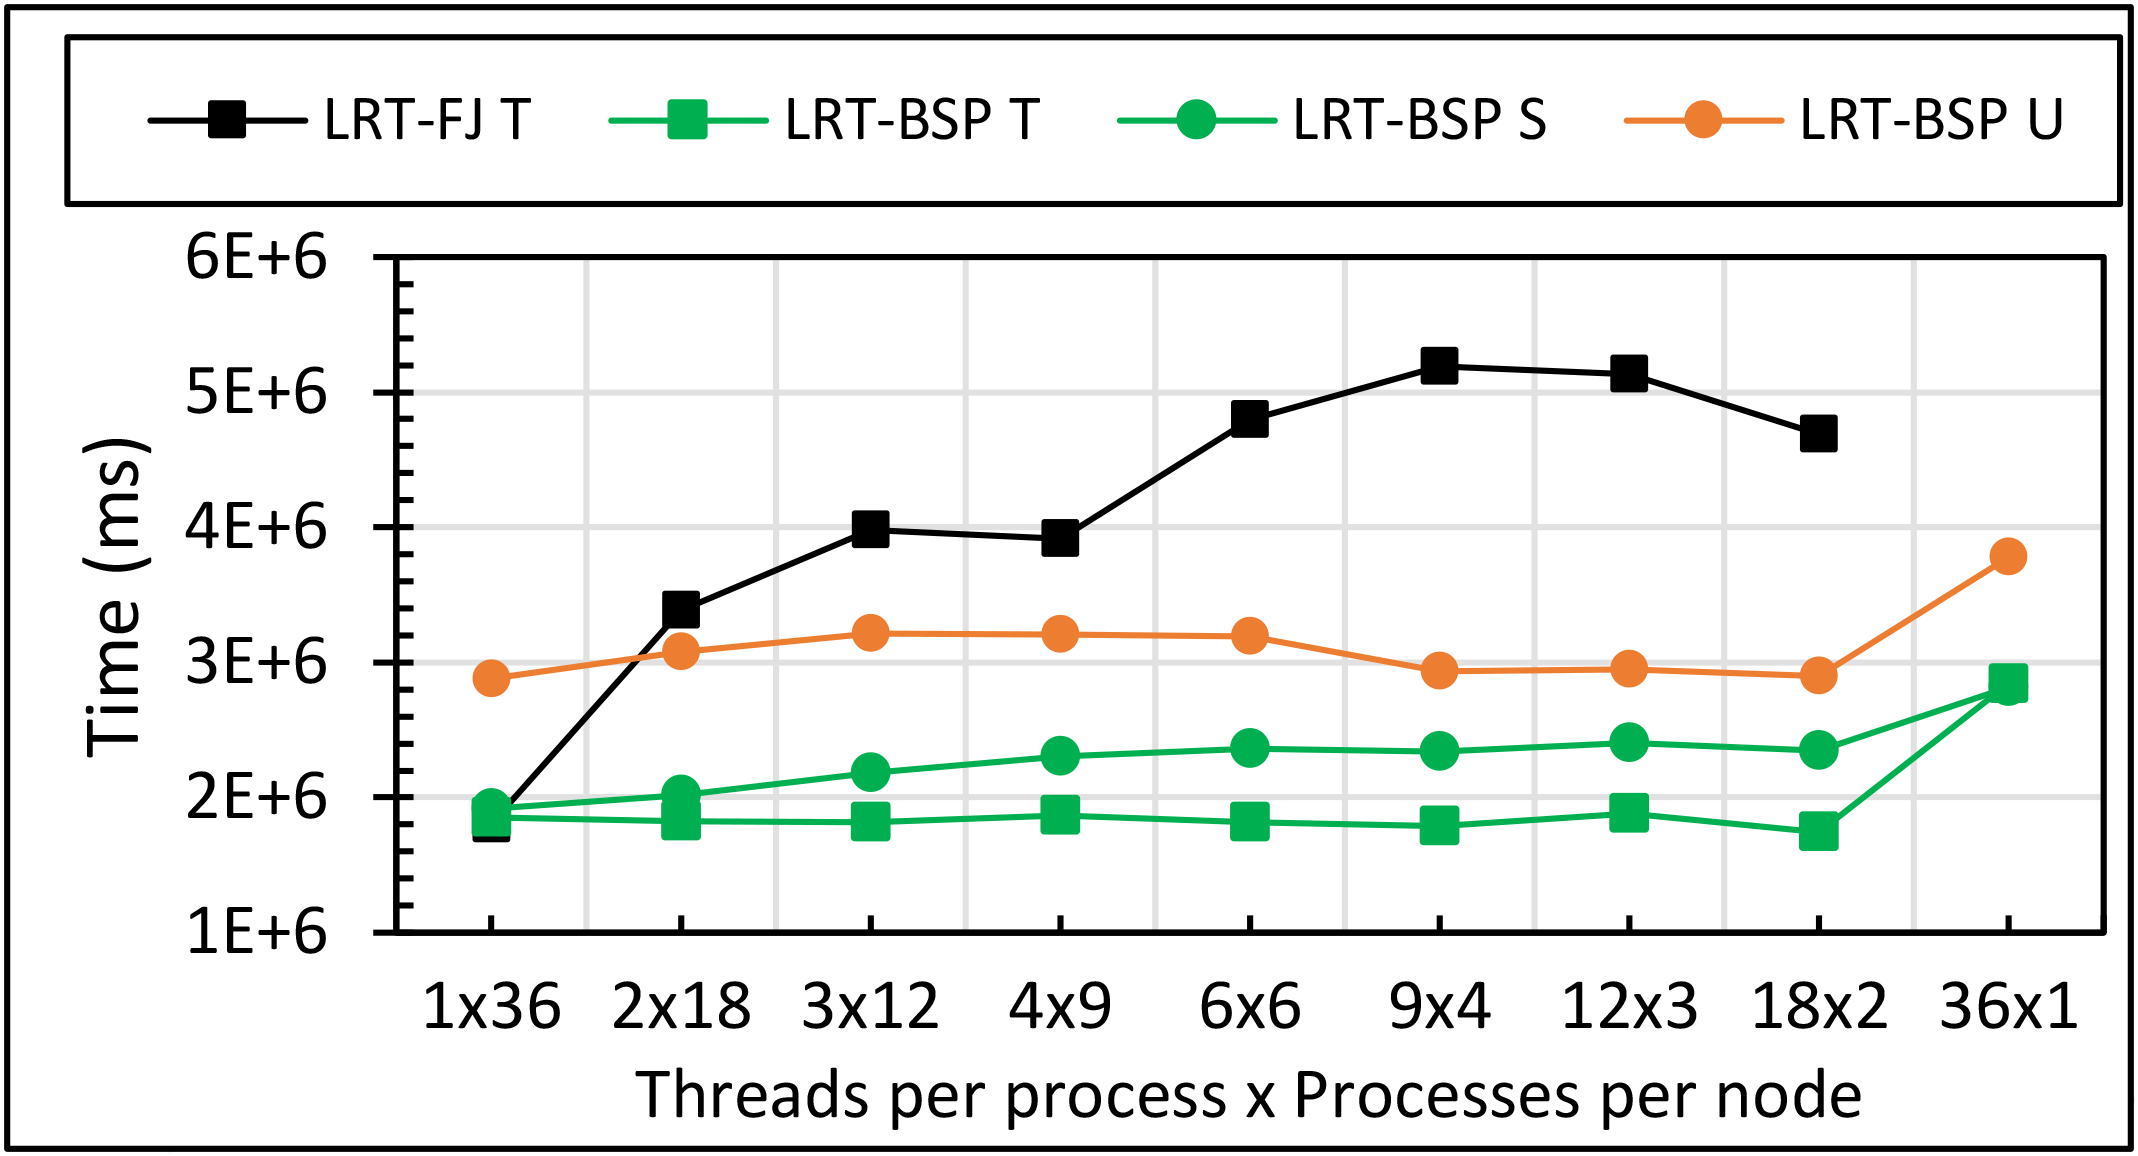
\includegraphics[width=1\columnwidth]{images/fig_damds_200k_binding_patterns_on_36core_nodes}
        \caption{Java DA-MDS 200k points performance on 16 of 36-core nodes for \ac{LRT-FJ} and \ac{LRT-BSP} over varying threads and processes. Affinity patterns are T,S,V, and U.}
        \label{fig:fig_damds_200k_binding_patterns_on_36core_nodes}
    \end{minipage}
\end{figure*}

%minipage kmeans flink vs spark vs mpi
\begin{figure*}[!htb]
	\begin{minipage}{0.49\textwidth}
        \centering
        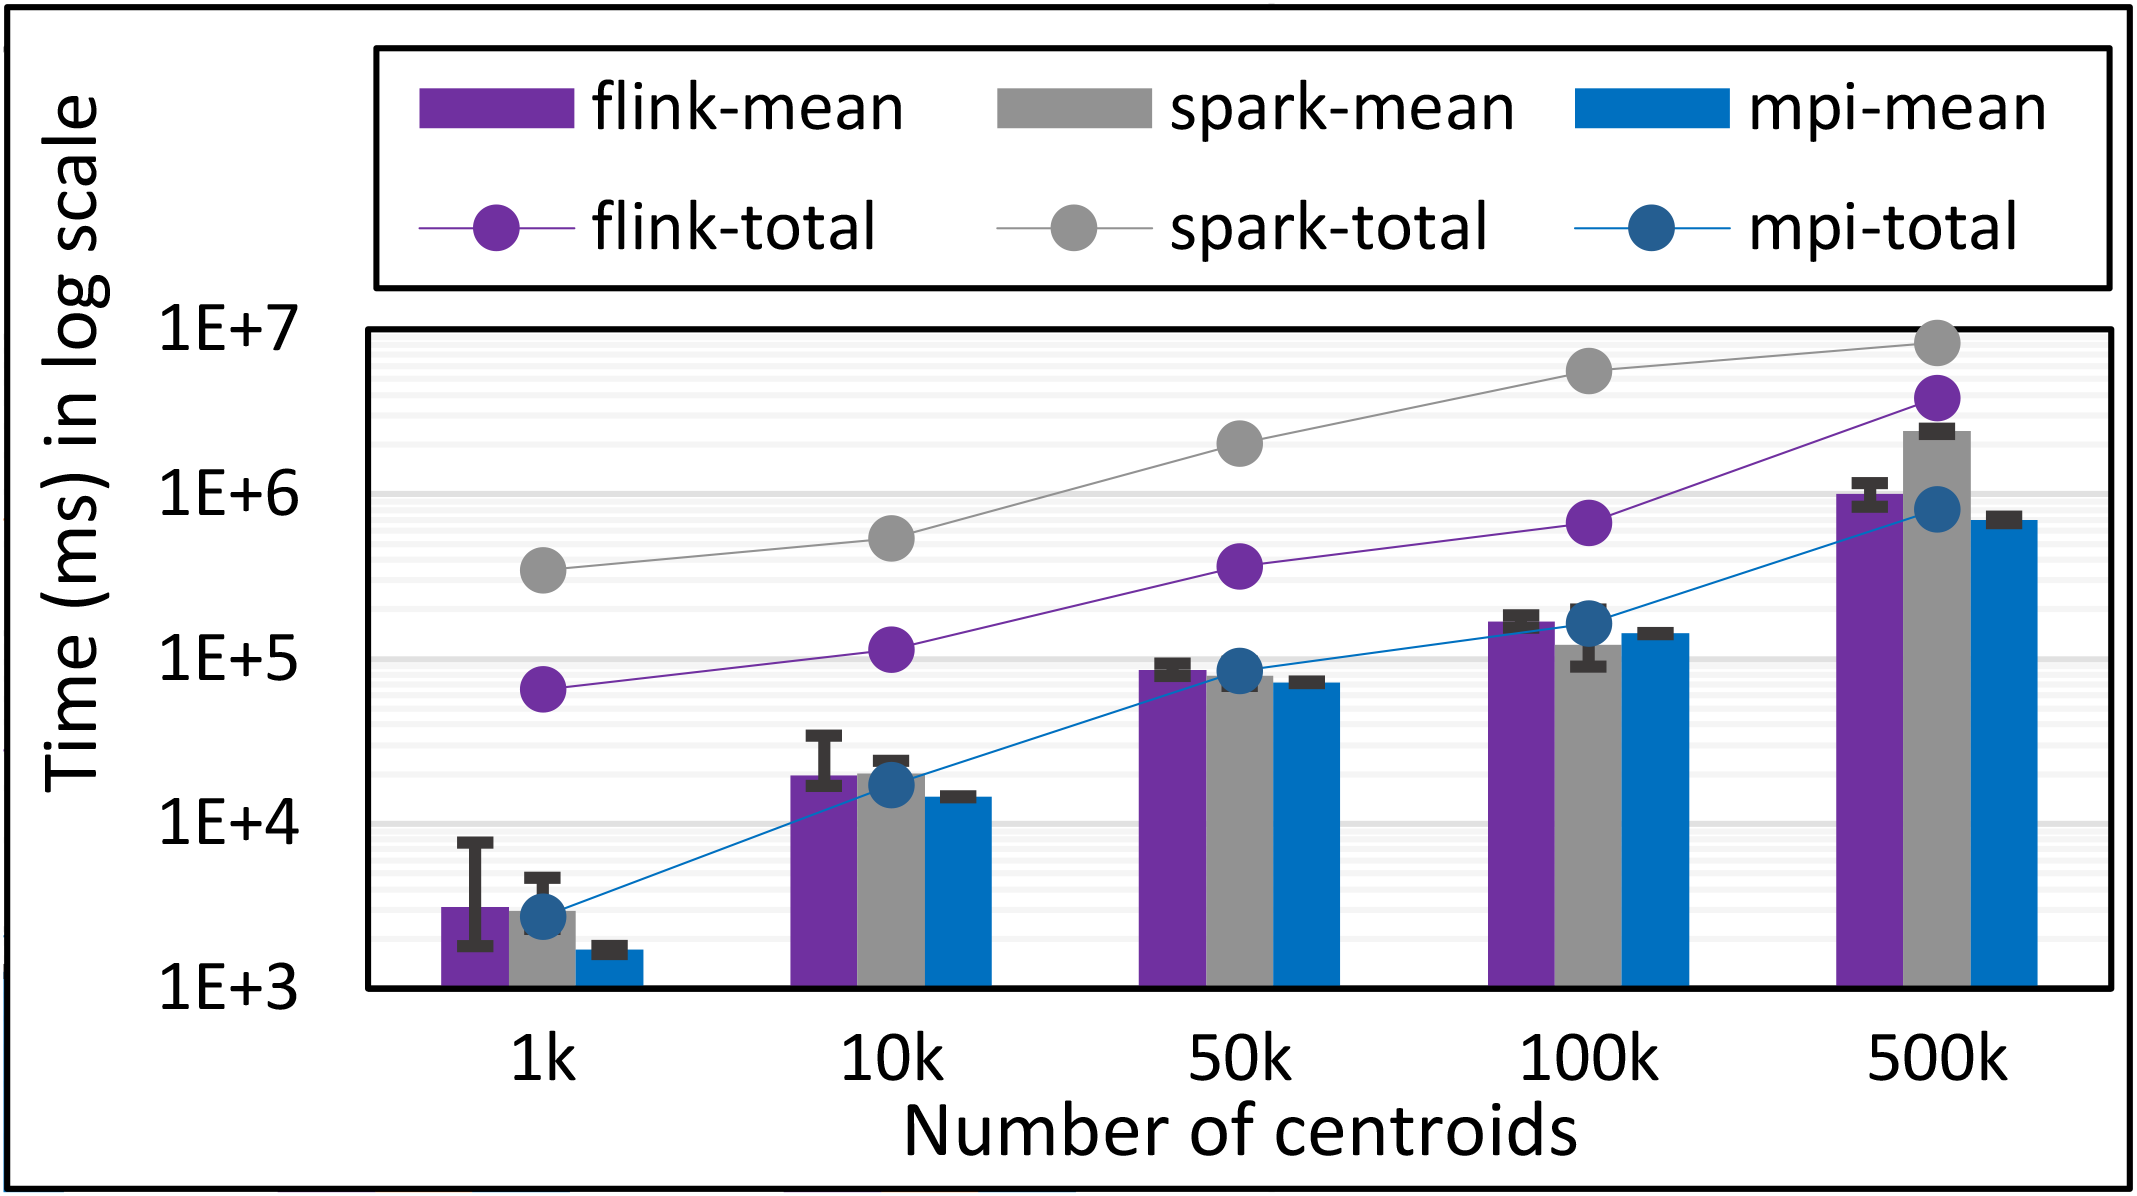
\includegraphics[width=1\columnwidth]{images/fig_kmeans_1mil_varying_centers_Flink_Spark_MPI}
        \caption{K-Means total and compute times for 1 million 2D points and 1k,10,50k,100k, and 500k centroids for Spark, Flink, and \ac{MPI} Java \ac{LRT-BSP} \texttt{T}. Run on 16 nodes as 24x1.}
        \label{fig:fig_kmeans_1mil_varying_centers_Flink_Spark_MPI}
    \end{minipage}
    \hspace{1.4mm}
    \begin{minipage}{0.49\textwidth}
        \centering
        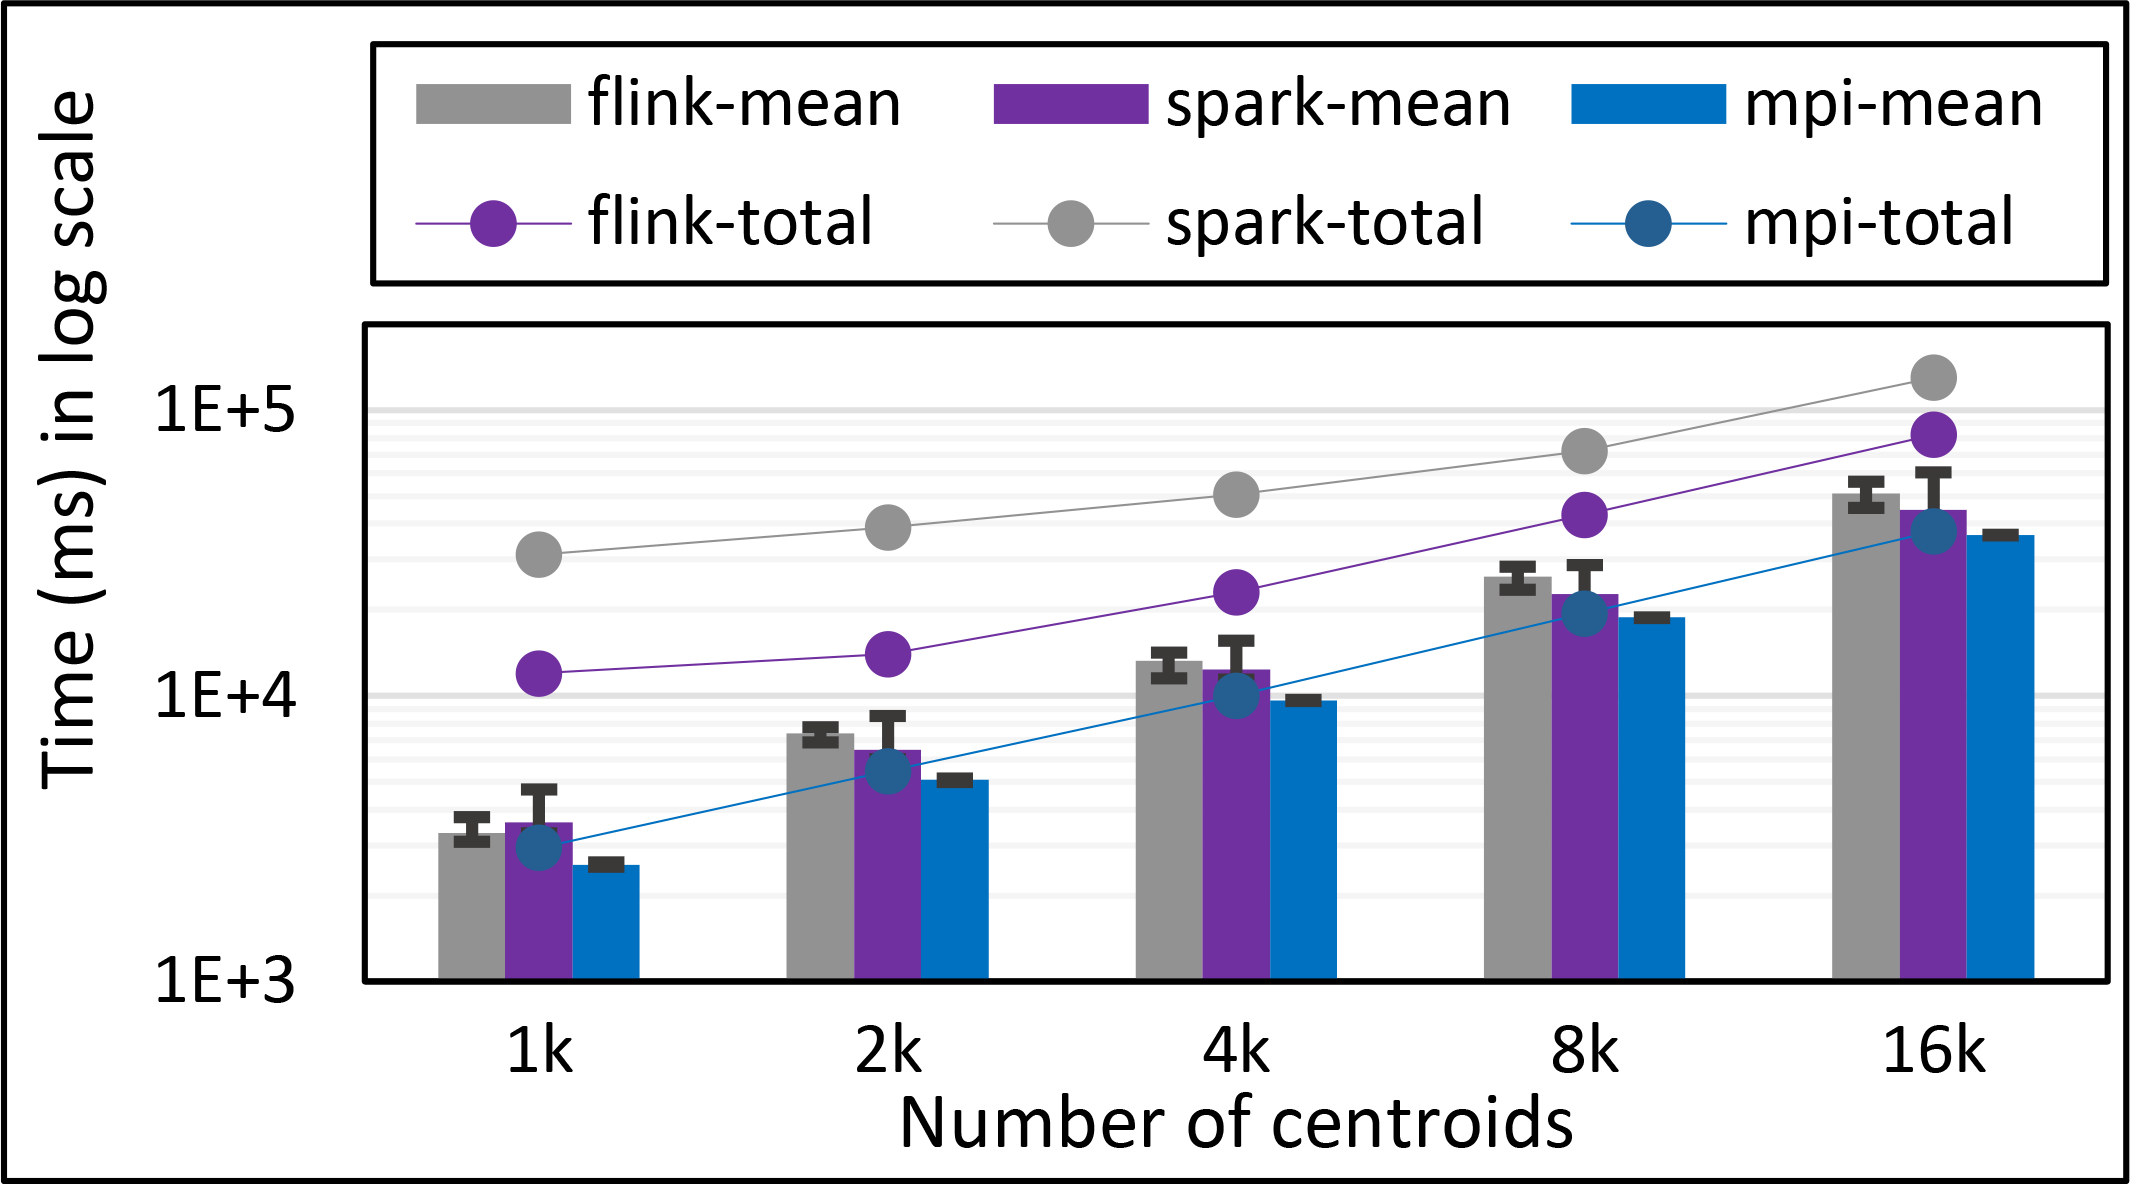
\includegraphics[width=1\columnwidth]{images/fig_kmeans_100k_varying_centers_Flink_Spark_MPI}
        \caption{K-Means total and compute times for 100k 2D points and 1k,2k,4k,8k, and 16k centroids for Spark, Flink, and \ac{MPI} Java \ac{LRT-BSP} \texttt{T}. Run on 1 node as 24x1}
        \label{fig:fig_kmeans_100k_varying_centers_Flink_Spark_MPI}
    \end{minipage}
\end{figure*}

%perf stat table for LRT-FJ vs LRT-BSP of 100k DA-MDS 18x2x32
\begin{table}[]
\centering
\caption{Linux \texttt{perf} statistics for \ac{DA-MDS} run of 18x2 on 32 nodes. Affinity pattern is \texttt{T}.}
\label{tbl:perf-stats}
\setlength\extrarowheight{4pt}
\begin{tabular}{l|r|r|}
\cline{2-3}
                                                & \multicolumn{1}{l|}{\textbf{LRT-FJ}} & \multicolumn{1}{l|}{\textbf{LRT-BSP}} \\ \hline
\multicolumn{1}{|l|}{\textbf{Context Switches}} & 477913                               & 31433                                 \\ \hline
\multicolumn{1}{|l|}{\textbf{CPU Migrations}}   & 63953                                & 31433                                 \\ \hline
\multicolumn{1}{|l|}{\textbf{dTLB load misses}} & 17226323                             & 6493703                               \\ \hline
\end{tabular}
\end{table}


%speedup table
\begin{table}[]
\centering
\caption{Java \ac{DA-MDS} speedup for varying data sizes on 24-core and 36-core nodes. Red values indicate the suboptimal performance of \ac{LRT-FJ} model compared to \ac{LRT-BSP}. Ideally, these values should be similar to their immediate left cell values.}
\label{tbl:mds-speedup}
\setlength\tabcolsep{6pt}
\setlength\extrarowheight{4pt}
\begin{tabular}{@{}c@{}|@{}C@{}|@{}C@{}|@{}C@{}|@{}C@{}|@{}C@{}|@{}C@{}|@{}C@{}|@{}C@{}|@{}C@{}|}
\cline{2-10}
                                     & \multicolumn{9}{c|}{\textbf{Data Size}}                                                                                                                                                                                              \\ \cline{2-10} 
\multicolumn{1}{c|}{}                & \multicolumn{3}{c|}{\textbf{50k}}                                          & \multicolumn{3}{c|}{\textbf{100k}}                                         & \multicolumn{3}{c|}{\textbf{200k}}                                         \\ \hline
\multicolumn{1}{|C|}{\textbf{24-Core Nodes}} & \textbf{1x24 LRT-BSP} & \textbf{12x2 LRT-BSP} & \textbf{12x2 LRT-FJ}       & \textbf{1x24 LRT-BSP} & \textbf{12x2 LRT-BSP} & \textbf{12x2 LRT-FJ}       & \textbf{1x24 LRT-BSP} & \textbf{12x2 LRT-BSP} & \textbf{12x2 LRT-FJ}       \\ \hline
\multicolumn{1}{|c|}{16}             & 1                     & 1                     & {\color[HTML]{FE0000} 0.6} & 1                     & 1                     & {\color[HTML]{FE0000} 0.6} & 1                     & 1                     & {\color[HTML]{FE0000} 0.4} \\ \hline
\multicolumn{1}{|c|}{32}             & 2.2                   & 2                     & {\color[HTML]{FE0000} 1.1} & 1.9                   & 1.9                   & {\color[HTML]{FE0000} 1.1} & 1.9                   & 2                     & {\color[HTML]{FE0000} 0.6} \\ \hline
\multicolumn{1}{|c|}{64}             & 3.9                   & 3.6                   & {\color[HTML]{FE0000} 1.9} & 3.6                   & 3.6                   & {\color[HTML]{FE0000} 1.9} & 3.7                   & 3.8                   & {\color[HTML]{FE0000} 0.9} \\ \hline
\multicolumn{1}{|C|}{\textbf{36-Core Nodes}} & \textbf{1x36 LRT-BSP} & \textbf{18x2 LRT-BSP} & \textbf{18x2 LRT-FJ}       & \textbf{1x36 LRT-BSP} & \textbf{18x2 LRT-BSP} & \textbf{18x2 LRT-FJ}       & \textbf{1x36 LRT-BSP} & \textbf{18x2 LRT-BSP} & \textbf{18x2 LRT-FJ}       \\ \hline
\multicolumn{1}{|c|}{16}             & 1                     & 1                     & {\color[HTML]{FE0000} 0.6} & 1                     & 1                     & {\color[HTML]{FE0000} 0.6} & 1                     & 1.1                   & {\color[HTML]{FE0000} 0.4} \\ \hline
\multicolumn{1}{|c|}{32}             & 2                     & 1.8                   & {\color[HTML]{FE0000} 0.9} & 1.9                   & 1.9                   & {\color[HTML]{FE0000} 1.1} & 1.9                   & 2.1                   & {\color[HTML]{FE0000} 0.6} \\ \hline
\end{tabular}
\end{table}

\begin{figure}
    \centering
    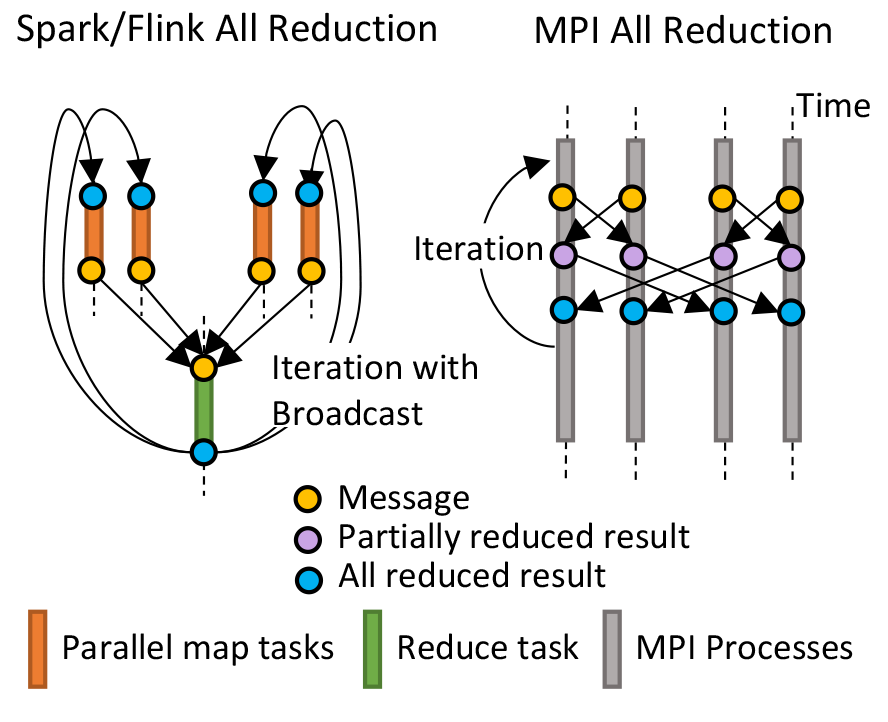
\includegraphics[width=0.9\columnwidth]{images/fig_flink_vs_mpi_reduction}
    \caption{Spark and Flink's all reduction vs \ac{MPI} all reduction.}
    \label{fig:fig_flink_vs_mpi_reduction}
\end{figure}



The experiments were run on Juliet, which is an Intel Haswell \ac{HPC} cluster with 128 nodes total. In this cluster 96 nodes have 24 cores (2 sockets x 12 cores each) and 32 nodes have 36 cores (2 sockets x 18 cores each) per node. Each node consists of 128GB of main memory and 56Gbps Infiniband interconnect and 1Gbps dedicated Ethernet connections. \ac{MPI} runs used the Infiniband except when comparing against Flink and Spark, where all three frameworks used \ac{TCP} communications.

\subsection{MPI Java and C K-Means}
\figurename~\ref{fig:fig_kmeans_1mil_1k_binding_patterns} and \figurename~\ref{fig:fig_C_kmeans_1mil_1k_binding_patterns} show K-Means Java and C total runtime for 1 million 2D points and 1000 centroids respectively. Each figure presents performance of both \ac{LRT-FJ} and \ac{LRT-BSP} models over the six binding patterns identified in Table ~\ref{tbl:affinity_patterns}. These were run on 24-core nodes; hence the abscissa shows all the eight possible combinations of threads and processes within a node to exploit the full 24-way parallelism. The left most pattern, 1x24, indicates all processes and the right most pattern, 24x1 indicates all threads within a node. Note, patterns 8x3 and 24x1 imply that processes span across \ac{NUMA} memory boundaries, which is known to be inefficient but presented here for completeness. The red and orange lines represent inherited thread affinity for \ac{LRT-FJ} and \ac{LRT-BSP} respectively. Similarly, the black and green lines illustrate explicit thread pinning, each to a core, for these two thread models. 

Java results suggest \ac{LRT-FJ} is the worst whatever the affinity strategy for any pattern other than 1x24, which is all \ac{MPI} and does not use thread parallel regions. A primary reason for this poor performance is the thread scheduling overhead in Java as \ac{FJ} threads are short-activated. Also, the \ac{JVM} spawns extra bookkeeping threads for \ac{GC} and other tasks, which compete for \acs{CPU} resources as well. Of the \ac{LRT-BSP} lines, the unbound threads (\texttt{U}) show the worst performance. Affinity patterns \texttt{S} and \texttt{T} seem to give the best runtime with increasing number of threads. 

C results show the same behavior for unbounded and explicitly bound threads. The two thread models, however, show similar performance, unlike Java. Further investigation of this behavior revealed OpenMP threads keep the \acsp{CPU} occupied at 100\% between \ac{FJ} regions suggesting OpenMP internally optimizes threads similar to the Java \ac{LRT-BSP} implementation introduced in this paper.

\figurename~\ref{fig:images/fig_kmeans_1mil_varying_centers_BSP_T_vs_BSP_S_Java} illustrates the effect of affinity patterns \texttt{T} and \texttt{S} for varying data sizes on \ac{LRT-BSP}. They performed similar to each other, but numbers favor pattern \texttt{T} over \texttt{S}.

\figurename~\ref{fig:images/fig_kmeans_1mil_varying_centers_BSP_T_C_vs_Java} compares Java and C \ac{LRT-BSP} runtimes for K-Means over varying data sizes across thread and process combinations. Results demonstrate Java performance is on par with C. Also, sometimes Java outperform C, mostly due to \ac{JIT} optimizations, as seen in the figure for 500k centers. 

\figurename~\ref{fig:fig_kmeans_1mil_varying_centers_by_10k_FJ_vs_BSP_T} and \figurename~\ref{fig:fig_kmeans_1mil_varying_centers_as_50k_500k_FJ_vs_BSP_T} showcase \ac{LRT-FJ} and \ac{LRT-BSP} performance over varying data sizes for affinity pattern \texttt{T}. In \figurename~\ref{fig:fig_kmeans_1mil_varying_centers_by_10k_FJ_vs_BSP_T}, the number of centroids were incremented as 1k,10k, and 100k. \ac{LRT-BSP} shows constant performance across thread and process combinations for all data sizes, where as \ac{LRT-FJ} exhibits abysmal performance with increasing threads and data sizes. \figurename~\ref{fig:fig_kmeans_1mil_varying_centers_as_50k_500k_FJ_vs_BSP_T} replicates the same experiment for data sizes 50k and 500k. Again, the results agree with those of \figurename~\ref{fig:fig_kmeans_1mil_varying_centers_by_10k_FJ_vs_BSP_T}.

\subsection{MPI Java \ac{MDS}}
\figurename~\ref{fig:fig_damds_50k_binding_patterns} through \figurename~\ref{fig:fig_damds_200k_binding_patterns_on_36core_nodes} illustrate \ac{DA-MDS} performance for data sizes 50k, 100k, and 200k on 24-core and 36-core nodes. Each figure presents \ac{DA-MDS} runtime for the two thread models and affinity patterns \texttt{T}, \texttt{V}, \texttt{S}, and \texttt{U}. Patterns \texttt{Q} and \texttt{R} were omitted as they showed similar abysmal performance as \texttt{U} in earlier K-Means results. Thread and process combinations for 24-core nodes are as same as the ones used in K-Means experiments. On 36-core nodes, nine patterns were tested from 1x36 to 36x1. However, as \ac{LRT-BSP} allocates data for all threads at process level, 200k decomposition over 16 nodes produced more data than what Java 1D arrays could hold. Therefore, this pattern could not be tested for 200k data. \ac{LRT-BSP} did not face this situation as data structures are local to threads and each allocates only data required for the thread, which is within Java's array limit of $2^{31} - 1$ elements.

The above results confirm that Java \ac{LRT-FJ} has the lowest performance irrespective of the binding, data size or the number of threads. On the other hand, the \ac{LRT-BSP} model produced constant high performance across all these parameters. Investigating these effects further, an 18x2 run for 100k data produced the \texttt{perf} stats in Table~\ref{tbl:perf-stats}, which show a vast number of context switches, \acs{CPU} migrations, and \acl{dTLB} load misses for \ac{LRT-FJ} compared to \ac{LRT-FJ}. These statistics are directly related with performance and hence explain the poor performance of \ac{LRT-FJ} model.

Table~\ref{tbl:mds-speedup} presents scaling of \ac{DA-MDS} across nodes for data sizes 50k, 100k, and 200k. Speedup values are measured against the all process -- 1x24 or 1x36 -- base case. With doubling of the nodes, the performance is expected to double. However, none of the 12x2 \ac{LRT-FJ} values came close to the expected number; hence shown in red.  In contrast, 12x2 of \ac{LRT-BSP} follows the expected doubling in performance and also can produce slightly better results than 1x24 with increasing data.

\subsection{Flink and Spark K-Means}
We evaluated the performance of K-Means algorithm implemented in Flink and Spark to compare these frameworks against \ac{MPI}. The evaluation was done in 16 nodes, each with 24 cores. We measured the difference between total time and computation time to estimate overheads including communication. Note, in both Spark and Flink, communications are handled intenally to the framework and it is not possible to measure this through the available \ac{API} functions. The results are shown in \figurename~\ref{fig:fig_kmeans_1mil_varying_centers_Flink_Spark_MPI} for 1 million 2D data points with varying number of centroids. We observed significant communication overhead in these frameworks compared to \ac{MPI}. The primary reason for such poor performance is the sub-optimal implementation of reductions in Flink and Spark.

\figurename~\ref{fig:fig_flink_vs_mpi_reduction} illustrates the dataflow reduction model implemented in Spark and Flink, where all parallel tasks send data to a single or multiple reduce tasks to perform the reduction. K-Means requires an \ac{MPI} like \texttt{Allreduce} semantics; hence the reduction in these programs is followed by a broadcast. Similar to the reduction operation, the broadcast is implemented serially as well. As the number of parallel tasks and the message size increase, this two-step approach becomes highly inefficient in performing global reductions. On the other hand, \ac{MPI} uses a recursive doubling algorithm for doing the reduction and broadcast together, which is very efficient and happens in-place. 

Since the communication overhead was dominant in K-Means algorithm, we performed a single node experiment with one process and multiple threads to look at computation costs more closely. With one process there is no network communication in Flink or Spark and \figurename~\ref{fig:fig_kmeans_100k_varying_centers_Flink_Spark_MPI} illustrates the results. Flink uses an actor-based execution model using Akka~\cite{gupta2012akka} framework to execute the tasks. The framework creates and destroys \ac{LRT-FJ} style threads to execute the individual tasks. Spark uses an executor/task model where an executor creates at most a single task for each core that is allocated to the executor. With this experiment, we have observed execution time imbalances among the parallel tasks for both Spark and Flink. The same has been observed with the \ac{LRT-FJ} Java \ac{MPI} implementation of K-Means and we could minimize these effects in \ac{MPI} Java with the \ac{LRT-BSP} style executions. Balanced parallel computations are vital to efficient parallel algorithms as the slowest task dominates the parallel computation time. 

% %perf stat table for LRT-FJ vs LRT-BSP of 100k DA-MDS 18x2x32
% \begin{table}[]
% \centering
% \caption{Linux \texttt{perf} statistics for \ac{DA-MDS} run of 18x2 on 32 nodes. Affinity pattern is \texttt{T}.}
% \label{tbl:perf-stats}
% \begin{tabular}{l|r|r|}
% \cline{2-3}
%                                                 & \multicolumn{1}{l|}{\textbf{LRT-FJ}} & \multicolumn{1}{l|}{\textbf{LRT-BSP}} \\ \hline
% \multicolumn{1}{|l|}{\textbf{Context Switches}} & 477913                               & 31433                                 \\ \hline
% \multicolumn{1}{|l|}{\textbf{CPU Migrations}}   & 63953                                & 31433                                 \\ \hline
% \multicolumn{1}{|l|}{\textbf{dTLB load misses}} & 17226323                             & 6493703                               \\ \hline
% \end{tabular}
% \end{table}


% %speedup table
% \begin{table}[]
% \centering
% \caption{Java \ac{DA-MDS} speedup for varying data sizes on 24-core and 36-core nodes. Red values indicate the suboptimal performance of \ac{LRT-FJ} model compared to \ac{LRT-BSP}. Ideally, these values should be similar to their immediate left cell values.}
% \label{tbl:mds-speedup}
% \setlength\tabcolsep{6pt}
% \setlength\extrarowheight{4pt}
% \begin{tabular}{@{}c@{}|@{}C@{}|@{}C@{}|@{}C@{}|@{}C@{}|@{}C@{}|@{}C@{}|@{}C@{}|@{}C@{}|@{}C@{}|}
% \cline{2-10}
%                                      & \multicolumn{9}{c|}{\textbf{Data Size}}                                                                                                                                                                                              \\ \cline{2-10} 
% \multicolumn{1}{c|}{}                & \multicolumn{3}{c|}{\textbf{50k}}                                          & \multicolumn{3}{c|}{\textbf{100k}}                                         & \multicolumn{3}{c|}{\textbf{200k}}                                         \\ \hline
% \multicolumn{1}{|C|}{\textbf{24-Core Nodes}} & \textbf{1x24 LRT-BSP} & \textbf{12x2 LRT-BSP} & \textbf{12x2 LRT-FJ}       & \textbf{1x24 LRT-BSP} & \textbf{12x2 LRT-BSP} & \textbf{12x2 LRT-FJ}       & \textbf{1x24 LRT-BSP} & \textbf{12x2 LRT-BSP} & \textbf{12x2 LRT-FJ}       \\ \hline
% \multicolumn{1}{|c|}{16}             & 1                     & 1                     & {\color[HTML]{FE0000} 0.6} & 1                     & 1                     & {\color[HTML]{FE0000} 0.6} & 1                     & 1                     & {\color[HTML]{FE0000} 0.4} \\ \hline
% \multicolumn{1}{|c|}{32}             & 2.2                   & 2                     & {\color[HTML]{FE0000} 1.1} & 1.9                   & 1.9                   & {\color[HTML]{FE0000} 1.1} & 1.9                   & 2                     & {\color[HTML]{FE0000} 0.6} \\ \hline
% \multicolumn{1}{|c|}{64}             & 3.9                   & 3.6                   & {\color[HTML]{FE0000} 1.9} & 3.6                   & 3.6                   & {\color[HTML]{FE0000} 1.9} & 3.7                   & 3.8                   & {\color[HTML]{FE0000} 0.9} \\ \hline
% \multicolumn{1}{|C|}{\textbf{36-Core Nodes}} & \textbf{1x36 LRT-BSP} & \textbf{18x2 LRT-BSP} & \textbf{18x2 LRT-FJ}       & \textbf{1x36 LRT-BSP} & \textbf{18x2 LRT-BSP} & \textbf{18x2 LRT-FJ}       & \textbf{1x36 LRT-BSP} & \textbf{18x2 LRT-BSP} & \textbf{18x2 LRT-FJ}       \\ \hline
% \multicolumn{1}{|c|}{16}             & 1                     & 1                     & {\color[HTML]{FE0000} 0.6} & 1                     & 1                     & {\color[HTML]{FE0000} 0.6} & 1                     & 1.1                   & {\color[HTML]{FE0000} 0.4} \\ \hline
% \multicolumn{1}{|c|}{32}             & 2                     & 1.8                   & {\color[HTML]{FE0000} 0.9} & 1.9                   & 1.9                   & {\color[HTML]{FE0000} 1.1} & 1.9                   & 2.1                   & {\color[HTML]{FE0000} 0.6} \\ \hline
% \end{tabular}
% \end{table}

\section{Discussion}\label{sec:discussion}
Spark and Flink are widely used efficient Big Data platforms for processing large amounts of data as well as executing machine learning algorithms. Both are in-memory computation platforms, unlike Hadoop, which is primarily a disk-based platform. These systems are designed to handle large amounts of data and be fault tolerant in case of failures. They can use disks as an auxiliary storage if the data is too large to fit in the memory. 

On the other hand, \ac{MPI} is a lightweight framework with excellent communication and execution semantics that are well suited for high performance multicore clusters. We believe Java \ac{MPI} implementations with careful design of threading, computations and communications as discussed in this work, provide top-notch performance for Java-based machine learning applications that match C implementations for big data platforms. This study shows the many factors that are critical for achieving the best possible performance and scalability and how they can be carefully tuned. 

Current implementations of Big Data computation frameworks lack efficient communication algorithms as implemented \ac{MPI}. We have identified inefficient communication as the most detrimental feature in getting to the best possible performance with Spark and Flink. For example, a carefully tuned broadcast operation can work in $O(log\ n)$ steps while a sequential implementation needs $O(n)$ where $n$ is the number of parallel communicators. As the parallelism increases the communication overhead in terms of both latency and bandwidth dramatically increases for the sequential approach compared to the optimized approach.

The computation time variations in the parallel tasks of Flink and Spark frameworks can be attributed to the \ac{LRT-FJ} style invocations and \acp{GC}. It is hard to completely avoid \ac{GC} overheads but Flink-like systems have adopted off-heap memory management for reducing this effect. The \ac{LRT-BSP} style threads can also help in reducing the compute time variations, as evident in \ac{MPI} Java applications. Another factor that can affect computation is the inefficient use of memory hierarchy. If cache optimizations are not considered, performance can show degrade drastically. Also, for larger data sets, it can be efficient to run multiple processes rather than a single process with threads due to large page tables required for the single process.   

It is also noteworthy that Scala~\cite{scalalang} plays a major role in Big Data frameworks such as Spark and Flink. Spark is developed with Scala, and provides \ac{API}'s for Java, Python and R in addition to Scala. Flink is developed with a mixture of Java and Scala, and provides a Scala \ac{API} in addition to its Java \ac{API}. Scala is a functional programming language that runs on the \ac{JVM}, this allows Scala to seamlessly work with Java libraries. Our results are of course sensitive to virtual machine used and not the language.


\section{Related Work} \label{sec:related}
A plethora of libraries are available for Java in \ac{HPC} environments including many \ac{MPI} implementations; Guillermo et al.~\cite{taboada2013java} discuss the performance of some of these frameworks in \ac{HPC} environments. MPJ-Express~\cite{baker2006mpj} and JaMP~\cite{klemm2007jamp} are popular pure Java implementation of the \ac{MPI} standard. In our work, we used OpenMPI's Java bindings to develop the \ac{MPI} applications. Our preliminary studies showed OpenMPI performed the best among the available Java \ac{MPI} implementations. Rajesh et al.~\cite{karmani2009actor} discusses actor-based frameworks to exploit the multicore machines and Flink uses actor model for handling concurrency. Java Garbage Collection (\ac{GC}) plays a vital role in \ac{HPC} Java applications because of the slowest parallel tasks dominating the performance. Maria et al.~\cite{carpen2015performance} shows how to optimize the Java \ac{GC} in multicore \ac{NUMA} machines. Research on improving Spark performance by introducing its own memory management and cache handing system is being done in Project Tungsten~\cite{tungsten}, which aims to greatly reduce the usage of java objects and to reduce Spark's memory footprint. 

Much research has been done on how to get better performance on multicore clusters using hybrid execution model of threads and processes~\cite{chorley2010performance, rabenseifner2009hybrid, camp2011streamline}. They discuss the performance across NUMA sockets, as well as how threads and processes perform in conjunction. In this work, we apply these techniques in the context of machine learning algorithms to get scalable performance.

Because of the high number of cores available in multicore nodes, hybrid communication models involving shared memory communication and network communication are preferred. In these models, the tasks within a node first communicate using shared memory and then the results are forwarded to other nodes in the cluster. Previous work by the authors~\cite{hpc2016:spidaljava} focused on improving the collective communications for Java machine learning algorithms using this hybrid approach. 

Hadoop~\cite{lam2010hadoop} became the first widely used system for big data processing and it uses a disk based communication among tasks with HDFS. Hadoop offers only the Map and Reduce  dataflow operations. The later systems such as Twiste~\cite{Ekanayake:2010:TRI:1851476.1851593}, Spark, Flink and Google Cloud Dataflow~\cite{akidau2015dataflow} are using in-memory and network communications among the tasks and are offering a rich set of data-flow operations compared to Hadoop. Bacause of the way communication is handled Spark and Flink, they are much closer to \ac{MPI} in run-time and can use the advanced communication features in MPI. 

These big data frameworks follow the  dataflow model and the equivalent of collective communications in \ac{MPI} are implemented as  dataflow operators. These implementations are elegant but inefficient compared to the optimized collective communication algorithms implemented in MPI~\cite{pjevsivac2007performance, thakur2005optimization}. Recent work by the authors~\cite{kamburugamuve2016towards} have improved communications of Apache Storm streaming framework with classical collective algorithms found in \ac{MPI} implementations. Harp~\cite{zhang2015harp} is a collective communication framework developed for Hadoop to speed up the machine learning applications. There has being efforts to bring HPC enhancements such as RDMA~\cite{lu2013high} to big data frameworks and these have given excellent performance in HPC environments.

Our findings are in the spirit of HPC-ABDS (the High Performance Computing enhanced Apache Big Data Stack)~\cite{kaleidoescope} and help establish a Big Data - HPC convergence approach~\cite{fox1858big}.

\section{Conclusion and Future Work} \label{sec:conclusion}
In this paper we discussed how to obtain consistent scalable performance of machine learning algorithms implemented in Java in large multicore clusters. The deficiencies in performance we observed before the improvements in Java \ac{MPI} machine learning applications can be observed on the current implementations of Big Data run-times such as Flink and Spark, and we are working on bringing these improvements to such frameworks. In particular we aim to improve the collective communications of Flink and Spark using efficient algorithms. As part of the SPIDAL (Scalable parallel interoperable data analytics library)~\cite{spidal-project} machine learning library we would like to apply these techniques to further algorithms.

% use section* for acknowledgement
\section*{Acknowledgment}
This work was partially supported by NSF CIF21 DIBBS 1443054 and NSF RaPyDLI 1415459. We thank Intel  for their support of the Juliet system, and extend our gratitude to the FutureSystems team for their support with the infrastructure. We also thank the Habanero Java team at Rice University for providing us access to their software. 

% trigger a \newpage just before the given reference
% number - used to balance the columns on the last page
% adjust value as needed - may need to be readjusted if
% the document is modified later
%\IEEEtriggeratref{8}
% The "triggered" command can be changed if desired:
%\IEEEtriggercmd{\enlargethispage{-5in}}

% references section

% can use a bibliography generated by BibTeX as a .bbl file
% BibTeX documentation can be easily obtained at:
% http://www.ctan.org/tex-archive/biblio/bibtex/contrib/doc/
% The IEEEtran BibTeX style support page is at:
% http://www.michaelshell.org/tex/ieeetran/bibtex/
%\bibliographystyle{IEEEtran}
% argument is your BibTeX string definitions and bibliography database(s)
%\bibliography{IEEEabrv,../bib/paper}
%
% <OR> manually copy in the resultant .bbl file
% set second argument of \begin to the number of references
% (used to reserve space for the reference number labels box)
% \begin{thebibliography}{1}

% \bibitem{IEEEhowto:kopka}
% H.~Kopka and P.~W. Daly, \emph{A Guide to \LaTeX}, 3rd~ed.\hskip 1em plus
%   0.5em minus 0.4em\relax Harlow, England: Addison-Wesley, 1999.

% \bibliography{2016.ieee.bigdata.bib}
% \end{thebibliography}

\balance
\bibliography{bibtex/IEEEabrv.bib,bibtex/IEEEref.bib}{}
\bibliographystyle{IEEEtran}


% that's all folks
\end{document}


